\chapter{Results}
	\section{Imaging Excited-State Dynamics}
		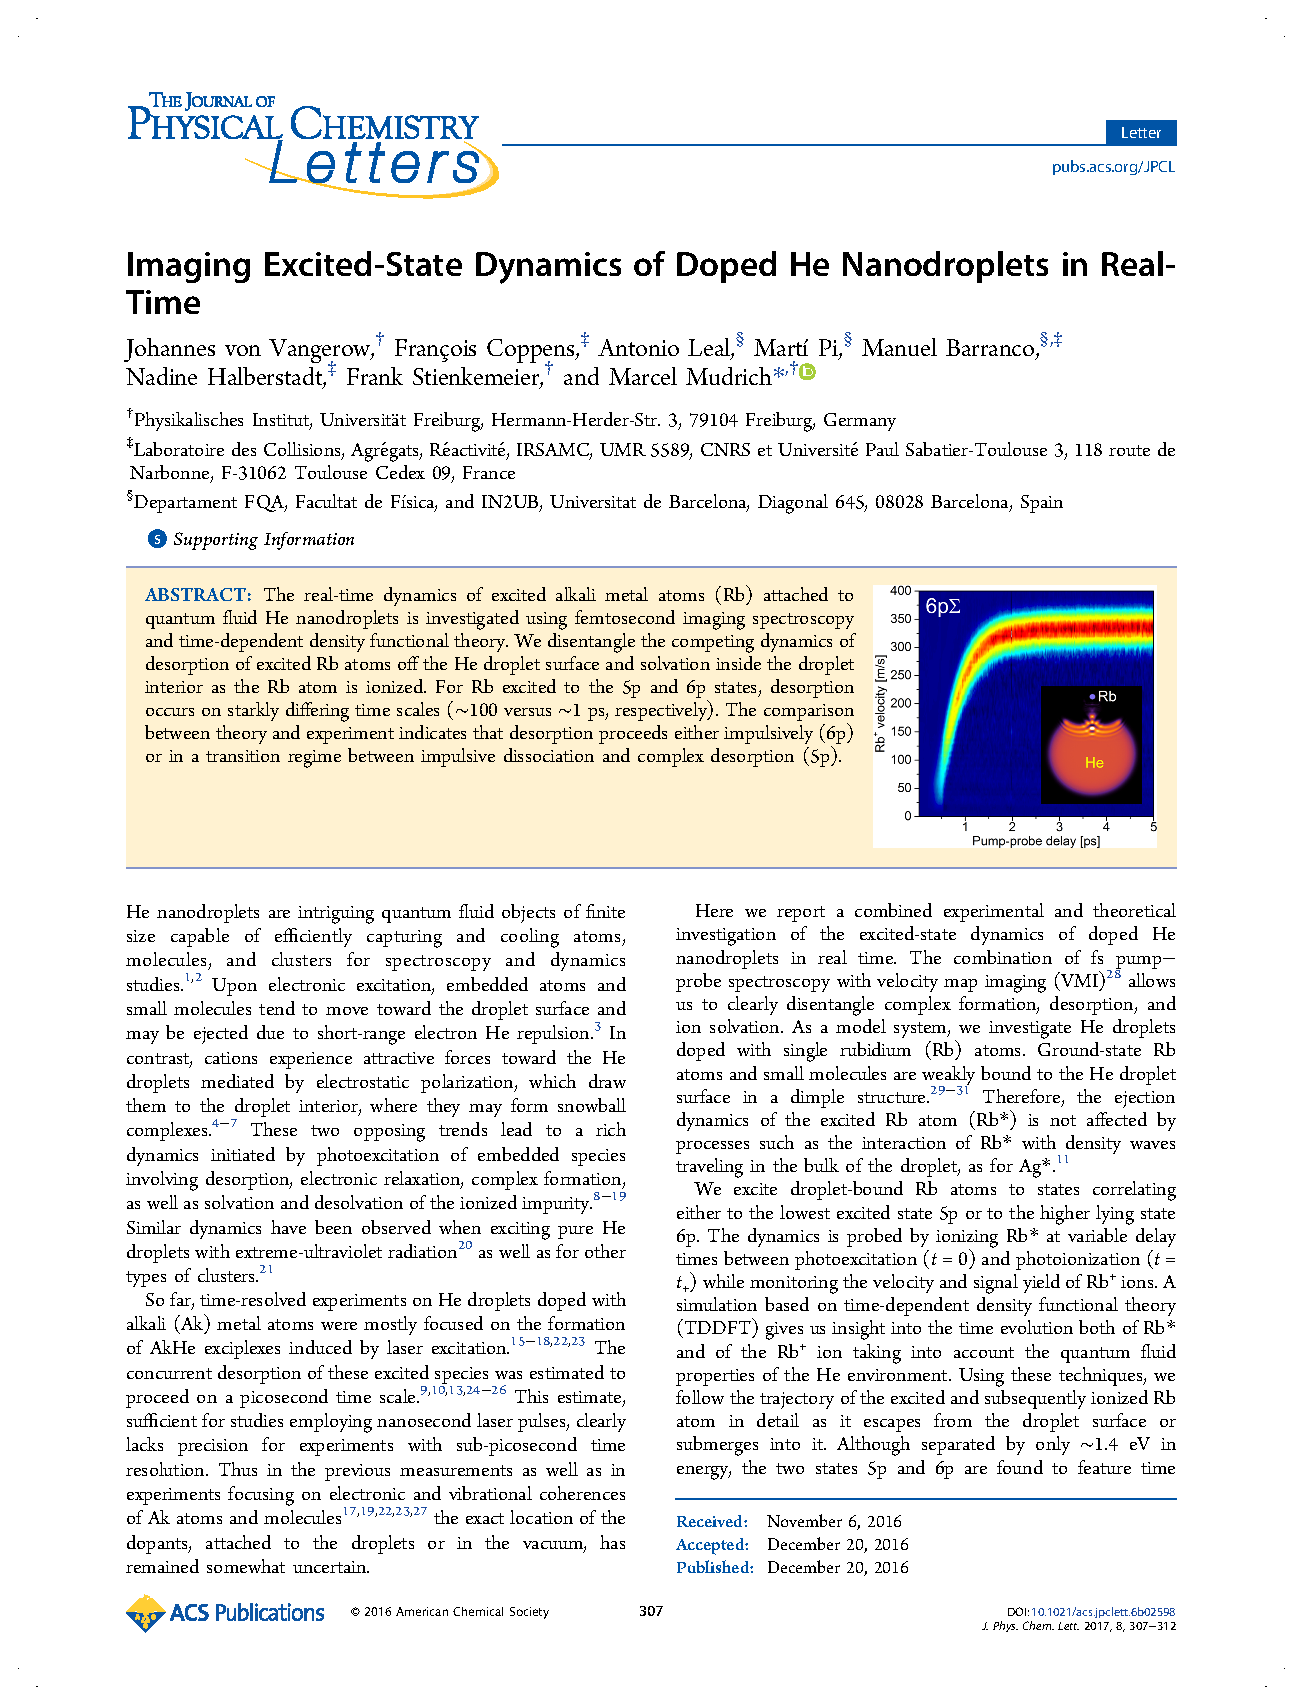
\includepdf[pages=-, scale=0.875, pagecommand={}]{jpcl_vol8_no1_pp307-312.pdf}

	\section{Desorption dynamics of RbHe exciplexes}
		\subsection{Time-resolved imaging spectroscopy}
		Typical experimental total electron and [RbHe]$^+$ ion VMIs recorded at a center wavelength of the pump laser pulse $\lambda=776$\,nm and a pump-probe delay of 2\,ns are shown in Figure~\ref{fig:VMI} a) and c), respectively. In these VMIs, the laser polarization is oriented along the $y$-axis. The corresponding electron energy distribution and ion speed distribution inferred from these images are presented in Figure~\ref{fig:VMI} b) and d), respectively. In addition, Figure~\ref{fig:VMI} b) contains photoelectron spectra measured at $\lambda=773$ and at $\lambda=794$\,nm. Note that the photoelectron spectra in Figure~\ref{fig:VMI} b) are rescaled in terms of electron binding energies $E_b=h\nu_2 - T_e$, where $h\nu_2=2hc/\lambda$ denotes the photon energy of the ionizing laser pulse and $T_e$ is the measured electron kinetic energy. The dashed vertical lines represent $E_b$ for free Rb atoms in their 5p$_{1/2}$ and 5p$_{3/2}$-states.

\begin{figure}[ht]
	\centering
	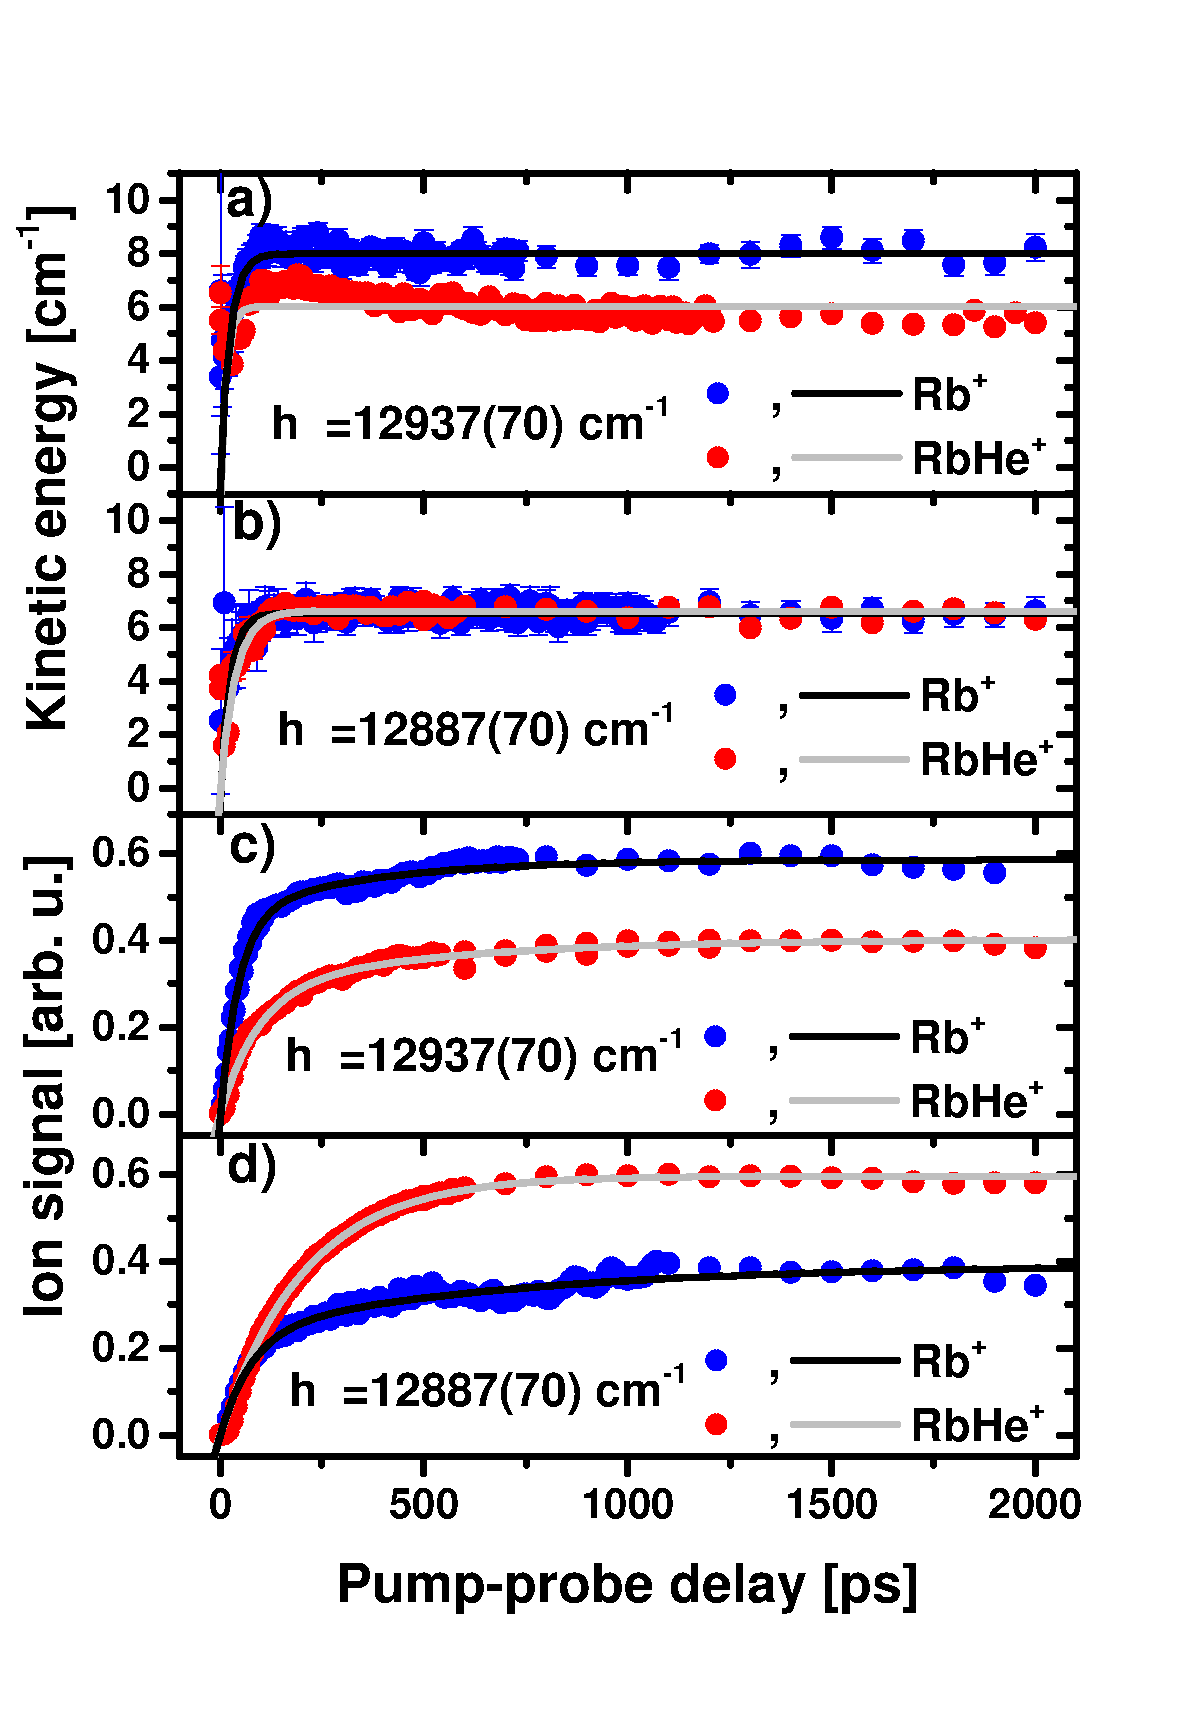
\includegraphics[width=0.9\linewidth]{fig3}
	\caption{Rb$^+$ and [RbHe]$^+$ ion kinetic energies [a) and b)] and signal yields [c) and d)] recorded at laser wavelengths $\lambda=773$~nm [12937~cm$^{-1}$, a) and c)] and $\lambda=776$~nm [12887~cm$^{-1}$, b) and d)].}
	\label{fig:speeds}
\end{figure}

\subsection{Photoion imaging}
The [RbHe]$^+$ ion distribution [Figure~\ref{fig:VMI} c)] is a round spot with a flat intensity distribution and a slight elongation in $x$-direction (perpendicular to the laser polarization). The corresponding speed distribution is broad and nearly symmetric. The red line depicts a skewed Gaussian distribution fitted to the data~\cite{mudholkar2000epsilon}. This fit is applied repeatedly to each speed distribution measured at various pump-probe delays in order to trace the evolution of the most probable kinetic energy, see Figure~\ref{fig:speeds} a) and b). The yields of ions, shown in Figure~\ref{fig:speeds} c) and d), are obtained by summing over ion counts contained in each image. Blue and red symbols show the results for Rb$^+$ and [RbHe]$^+$ ions, respectively. Both kinetic energies and ion yields monotonously increase within 100-500~ps, with a slight overshoot at $\lambda=773$~nm [Figure~\ref{fig:speeds} a)]. This increase results from the competing processes of desorption of the excited neutral Rb and RbHe species, and falling back of the Rb$^+$ and [RbHe]$^+$ photoions into the He droplet due to attractive Rb$^+$-He interactions, as discussed in Refs.~\cite{Vangerow:2015,Vangerow:2017}. By comparing the experimental data with TD-DFT simulations, we concluded that the 5p-correlated states of Rb and RbHe desorb off He droplets not purely impulsively, but in a more complex evaporation-like process~\cite{Vangerow:2017}. The overshoot of speeds in Figure~\ref{fig:speeds} a) is likely due to weak long-range attractive forces acting between the desorbing Rb and RbHe and the He droplet surface, which slightly slow down the relative motion in the later stage of desorption.

The data in Figure~\ref{fig:speeds} a) are measured at $\lambda=773$~nm (12937~cm$^{-1}$), which corresponds to the excitation of the RbHe complex into the 5p$\Sigma_{1/2}$-state, with some contribution of the 5p$\Pi_{3/2}$-state due to overlapping absorption bands and due to the broad spectral profile of the laser~\cite{Stienkemeier:1996,Bruehl:2001,Callegari:2011}. The 5p$\Sigma_{1/2}$-state is the most repulsive one out of the three states studied here. Accordingly, the asymptotic most probable speed of Rb$^+$ reached at long delays is comparatively high, $\hat{v}=85$~m/s, corresponding to a kinetic energy of $8~$cm$^{-1}$, whereas for [RbHe]$^+$ we find $\hat{v}=40$~m/s ($5.8~$cm$^{-1}$). Since the diatomic 5p$\Sigma_{1/2}$ RbHe potential is purely repulsive [Figure~\ref{fig:pots} a)], this component of the excited population results in the desorption of neat Rb atoms. Accordingly, the yield of detected Rb$^+$ ions exceeds that of [RbHe]$^+$ ions by about a factor 1.5. 
%{\bf *** Is there a good explanation why we measure [RbHe]$^+$ here at all? Is it due to the admixture of 5p$\Pi_{3/2}$, or does the 5p$\Sigma_{1/2}$ pseudodiatomic state also produce exciplexes? ***}

At $\lambda=$776~nm (12887~cm$^{-1}$), a higher contribution of the 5p$\Pi_{3/2}$-state is excited, which efficiently forms RbHe exciplexes~\cite{Bruehl:2001}. Thus, the yield of [RbHe]$^+$ ions is higher than that of Rb$^+$ by a factor 1.5. The Rb$^+$ and [RbHe]$^+$ asymptotic most probable speed is $\hat{v}=42$~m/s (6.3~cm$^{-1}$), close to that of [RbHe]$^+$ at $\lambda=773$\,nm. At $\lambda=794$~nm (12595~cm$^{-1}$), the 5p$\Pi_{1/2}$-state of the Rb-He droplet complex is excited (not shown), and no [RbHe]$^+$ ions are detected. Therefore we have recorded only Rb$^+$ ion images at that wavelength~\cite{Vangerow:2017}. Here, the Rb$^+$ asymptotic most probable speed is lowest, $\hat{v}=38$~m/s (5.1~cm$^{-1}$), because dopant-He repulsion is weaker.

The transient kinetic energies measured at all laser wavelengths rise within a delay time of about 500~ps. 
%At $\lambda=773$~nm ($12937$~cm$^{-1}$, mainly 5p$\Sigma_{1/2}$-excitation), the [RbHe]$^+$ kinetic energy exhibits a maximum at $t\sim 150~$ps. In addition, at this wavelength, the kinetic energy is significantly higher for Rb$^+$ than for [RbHe]$^+$, whereas for $\lambda=776~$nm (12887~cm$^{-1}$) the data nearly coincide. 
The characteristic energy rise time (to half value), $\tau^i_E$, and the asymptotic ion kinetic energy $E_\infty^I$, are determined by fitting the data with an exponential function
\begin{align} 
E^I(t)=E_\infty^I\cdot\left(1-\mathrm{exp}[-\ln2\cdot t/\tau^i_E]\right).\qquad
\label{E(t)}
\end{align} 
The resulting fit parameters are summarized in table~\ref{tab:FitParsIons}. 
 
The ion yields increase with pump-probe delay slightly more slowly than the ion kinetic energies, where the Rb$^+$ ion signal rises faster than the [RbHe]$^+$ ion signal at short delays. The initial fast rise of the Rb$^+$ ion yield flattens out at delays around 100~ps and continues to rise slightly up to about 2~ns. The [RbHe]$^+$ ion yields show a similar initial fast rise followed by a more pronounced slow increase that levels off somewhat earlier. Therefore, for fitting the Rb$^+$ and [RbHe]$^+$ ion yield data we use a biexponential function,
\begin{align} 
I(t)=A^i_1\cdot\left(1-\mathrm{exp}[-\ln2\cdot t/\tau^i_1]\right)+A^i_2\cdot\left(1-\mathrm{exp}[-\ln2\cdot t/\tau^i_2]\right),\qquad
\label{I_Rb}
\end{align}
where $(A^i_1,\tau^i_1$) and $(A^i_2,~\tau^i_2$) parametrize the fast and the slow signal rise, respectively.

%\begin{table}[ht]
%	\caption{Multi-column and multi-row table}
%	\begin{center}
%		\begin{tabular}{cccc}
%			\hline
%			\multicolumn{2}{c}{\multirow{2}{*}{Multi-col-row}}&X&X\\
%			\multicolumn{2}{c}{}&X&X\\
%			\hline
%			X&X&X&x\\
%			\hline
%		\end{tabular}
%	\end{center}
%	\label{tab:multicol}
%\end{table}

\begin{table*}[t]
%\begin{table}[H]
	\begin{center}
		\begin{tabular}{| c c | c | c c | c c c c| c |}
			\hline
			$\lambda$\,[nm] & State & Ion & $E_\infty^I$\,[1/cm] & $\tau^i_E$\,[ps] & $A^i_1$ & $\tau^i_1$\,[ps] & $A^i_2$ & $\tau^i_2$\,[ps] & $\beta$ \\  
			\hline\hline
			773 & $\Sigma_{1/2}/\Pi_{3/2}$ 	& Rb$^+$ & 8.0(1) & 17(1) & 0.45(2) & 32(1) & 0.14(2) & 234(33) & 0.17(1) \\
				& 							& [RbHe]$^+$ & 6.0(1) & 10(2) & 0.17(2) & 41(6) & 0.22(2) & 178(17) & 0.13(1) \\
			\hline
			776 & $\Pi_{3/2}/\Sigma_{1/2}$ & Rb$^+$ & 6.5(3) & 17(1) & 0.24(2) & 53(5) & 0.16(2) & 490(104) & -0.16(1) \\
			 &  & [RbHe]$^+$ & 6.6(3) & 26(1) & 0.60(1) & 143(2) & 0.00(1) & - & -0.39(1)  \\
			\hline
						780 & $\Pi_{3/2}$ &  [RbHe]$^+$ & 6.3(1) & 24(2) & 0.95(1) & 186(1) & 0.00(1) & - & 0.35(1) \\
			\hline
		\end{tabular}
		\caption{Time constants and energies inferred from pump-probe measurements of Rb$^+$ and [RbHe]$^+$ ion yields at the 5p$\Sigma_{1/2}$ and 5p$\Pi_{3/2}$-states of the Rb-He droplet complex, obtained from fits with equations (\ref{E(t)}) and (\ref{I_Rb}), see Figure \ref{fig:speeds}.
		\label{tab:FitParsIons}}
	\end{center}
\end{table*}
While neither the Rb$^+$ and [RbHe]$^+$ asymptotic energies $E_\infty^I$, nor the energy rise times $\tau^i_E$ depend much on $\lambda$, the rise times of ion yields of RbHe$^{+}$, $\tau^i_1$, clearly decrease monotonically with decreasing $\lambda$ (increasing photon energy) by a factor $6$, ranging from 186~ps at $\lambda=780$~nm to 32~ps at $\lambda=773$~nm. The trend that the dynamics proceeds faster with decreasing $\lambda$ (increasing photon energy) is partly due to the increasingly repulsive dopant-He interaction and agrees with our previous findings~\cite{Vangerow:2015,Vangerow:2017}. However, the observation that the ion yields rise more slowly than the ion kinetic energies cannot be understood with the concept of impulsive desorption and fall-back. In that model, ion kinetic energies should be affected by ion-He attraction up to long delay times exceeding the fall-back time. Note that in previous experiments on the Rb 6p-state, where desorption proceeded impulsively, ion energies indeed increased more slowly than ion yields~\cite{Vangerow:2017}. Therefore we take our current finding ($\tau^i_1, \,\tau^i_2 > \tau^i_E$) as a further indication for a non-impulsive, evaporation-like desorption mechanism. 

Furthermore, from our analysis of the VMIs we obtain information about the anisotropy of the ion angular distribution, characterized by the parameter $\beta$~\cite{Zare:1972}. For [RbHe]$^+$ at long delay times we find $\beta=-0.39(1)$ when a higher contribution of the $\Pi_{3/2}$-state is excited at $\lambda=776$~nm. At $\lambda=773$~nm (mainly $\Sigma_{1/2}$-excitation), the anisotropy becomes slightly positive, $\beta=0.13(1)$. The corresponding values for the Rb$^+$ ion distributions are $\beta=-0.16(1)$ and $\beta=0.17(1)$, respectively. While the signs of the $\beta$-values are in accordance with the symmetries of the pseudo-diatomic states (ideal perpendicular $\Sigma\rightarrow\Pi$-transition in a diatomic implies $\beta=-1$, parallel $\Sigma\rightarrow\Sigma$-transition implies $\beta=2$), the absolute values are much smaller. On the one hand, this is due to the mixing of excited $\Sigma_{1/2}$ and $\Pi_{3/2}$-states. On the other hand, the desorption process is significantly more complex than direct dissociation of a diatomic molecule. We recall that the $\beta$-values came much closer to the ideal values in the case of excitation of Rb to the high-lying 6p-correlated states, where desorption proceeded more impulsively~\cite{Fechner:2012,Vangerow:2014,Vangerow:2017}. 
%The larger absolute value of $\beta$ measured at $\lambda=776$~nm for [RbHe]$^+$ likely reflects the fact that RbHe exciplexes are formed from the $\Pi_{3/2}$-part of the excited state. The fact that 

%The data points roughly follow a linear trend 
%\begin{align}
%\tau(E)=209(12)\,\mathrm{ps}- E \cdot %1.5(2)\,\frac{\mathrm{ps}}{\mathrm{cm}^{-1}}. \qquad
%\end{align}
%The same fit of the rise times of Rb$^+$ ion yields results in an offset of 107(1)\,ps and a slope of -0.58(1)\,$\frac{\mathrm{ps}}{\mathrm{cm}^{-1}}$.

We mention that in earlier pump-probe experiments, significantly different Rb$^+$ and [RbHe]$^+$ ion yield curves were measured~\cite{Droppelmann:2004}. However, in those experiments, NIR light emitted directly from a mode-locked titanium:sapphire laser was used at a pulse repetition rate of 80~MHz. Therefore, a large fraction of the ion signals actually stemmed from Rb and RbHe that had been desorbed off the droplets by preceding pulse pairs. Thus, the observed pump-probe transients may have reflected the internal dynamics of free RbHe instead of the dynamics of the Rb-He droplet interaction. Besides, near-resonant two-photon excitation of higher lying states correlating to the Rb 5d-level were probably involved in the observed dynamics. This raises some doubts as to the conclusions of those previous experiments in terms of exciplex formation times~\cite{Droppelmann:2004,Vangerow:2017}. Further studies are needed to clarify this issue.

From the overall resemblance of the [RbHe]$^+$ and Rb$^+$ kinetic energy curves and ion yields in the present study one is tempted to conclude that RbHe exciplex formation is fast and desorption of RbHe off the He droplet surface proceeds essentially in the same way as for neat Rb atoms. However, the more pronounced biexponential rise of [RbHe]$^+$ ion yields, as well as complementary delay-dependent photoelectron measurements, and numerical simulations presented in the following sections will show that the desorption dynamics of RbHe exciplexes actually is more complex than that of Rb atoms.

\begin{figure}[ht]
	\centering
	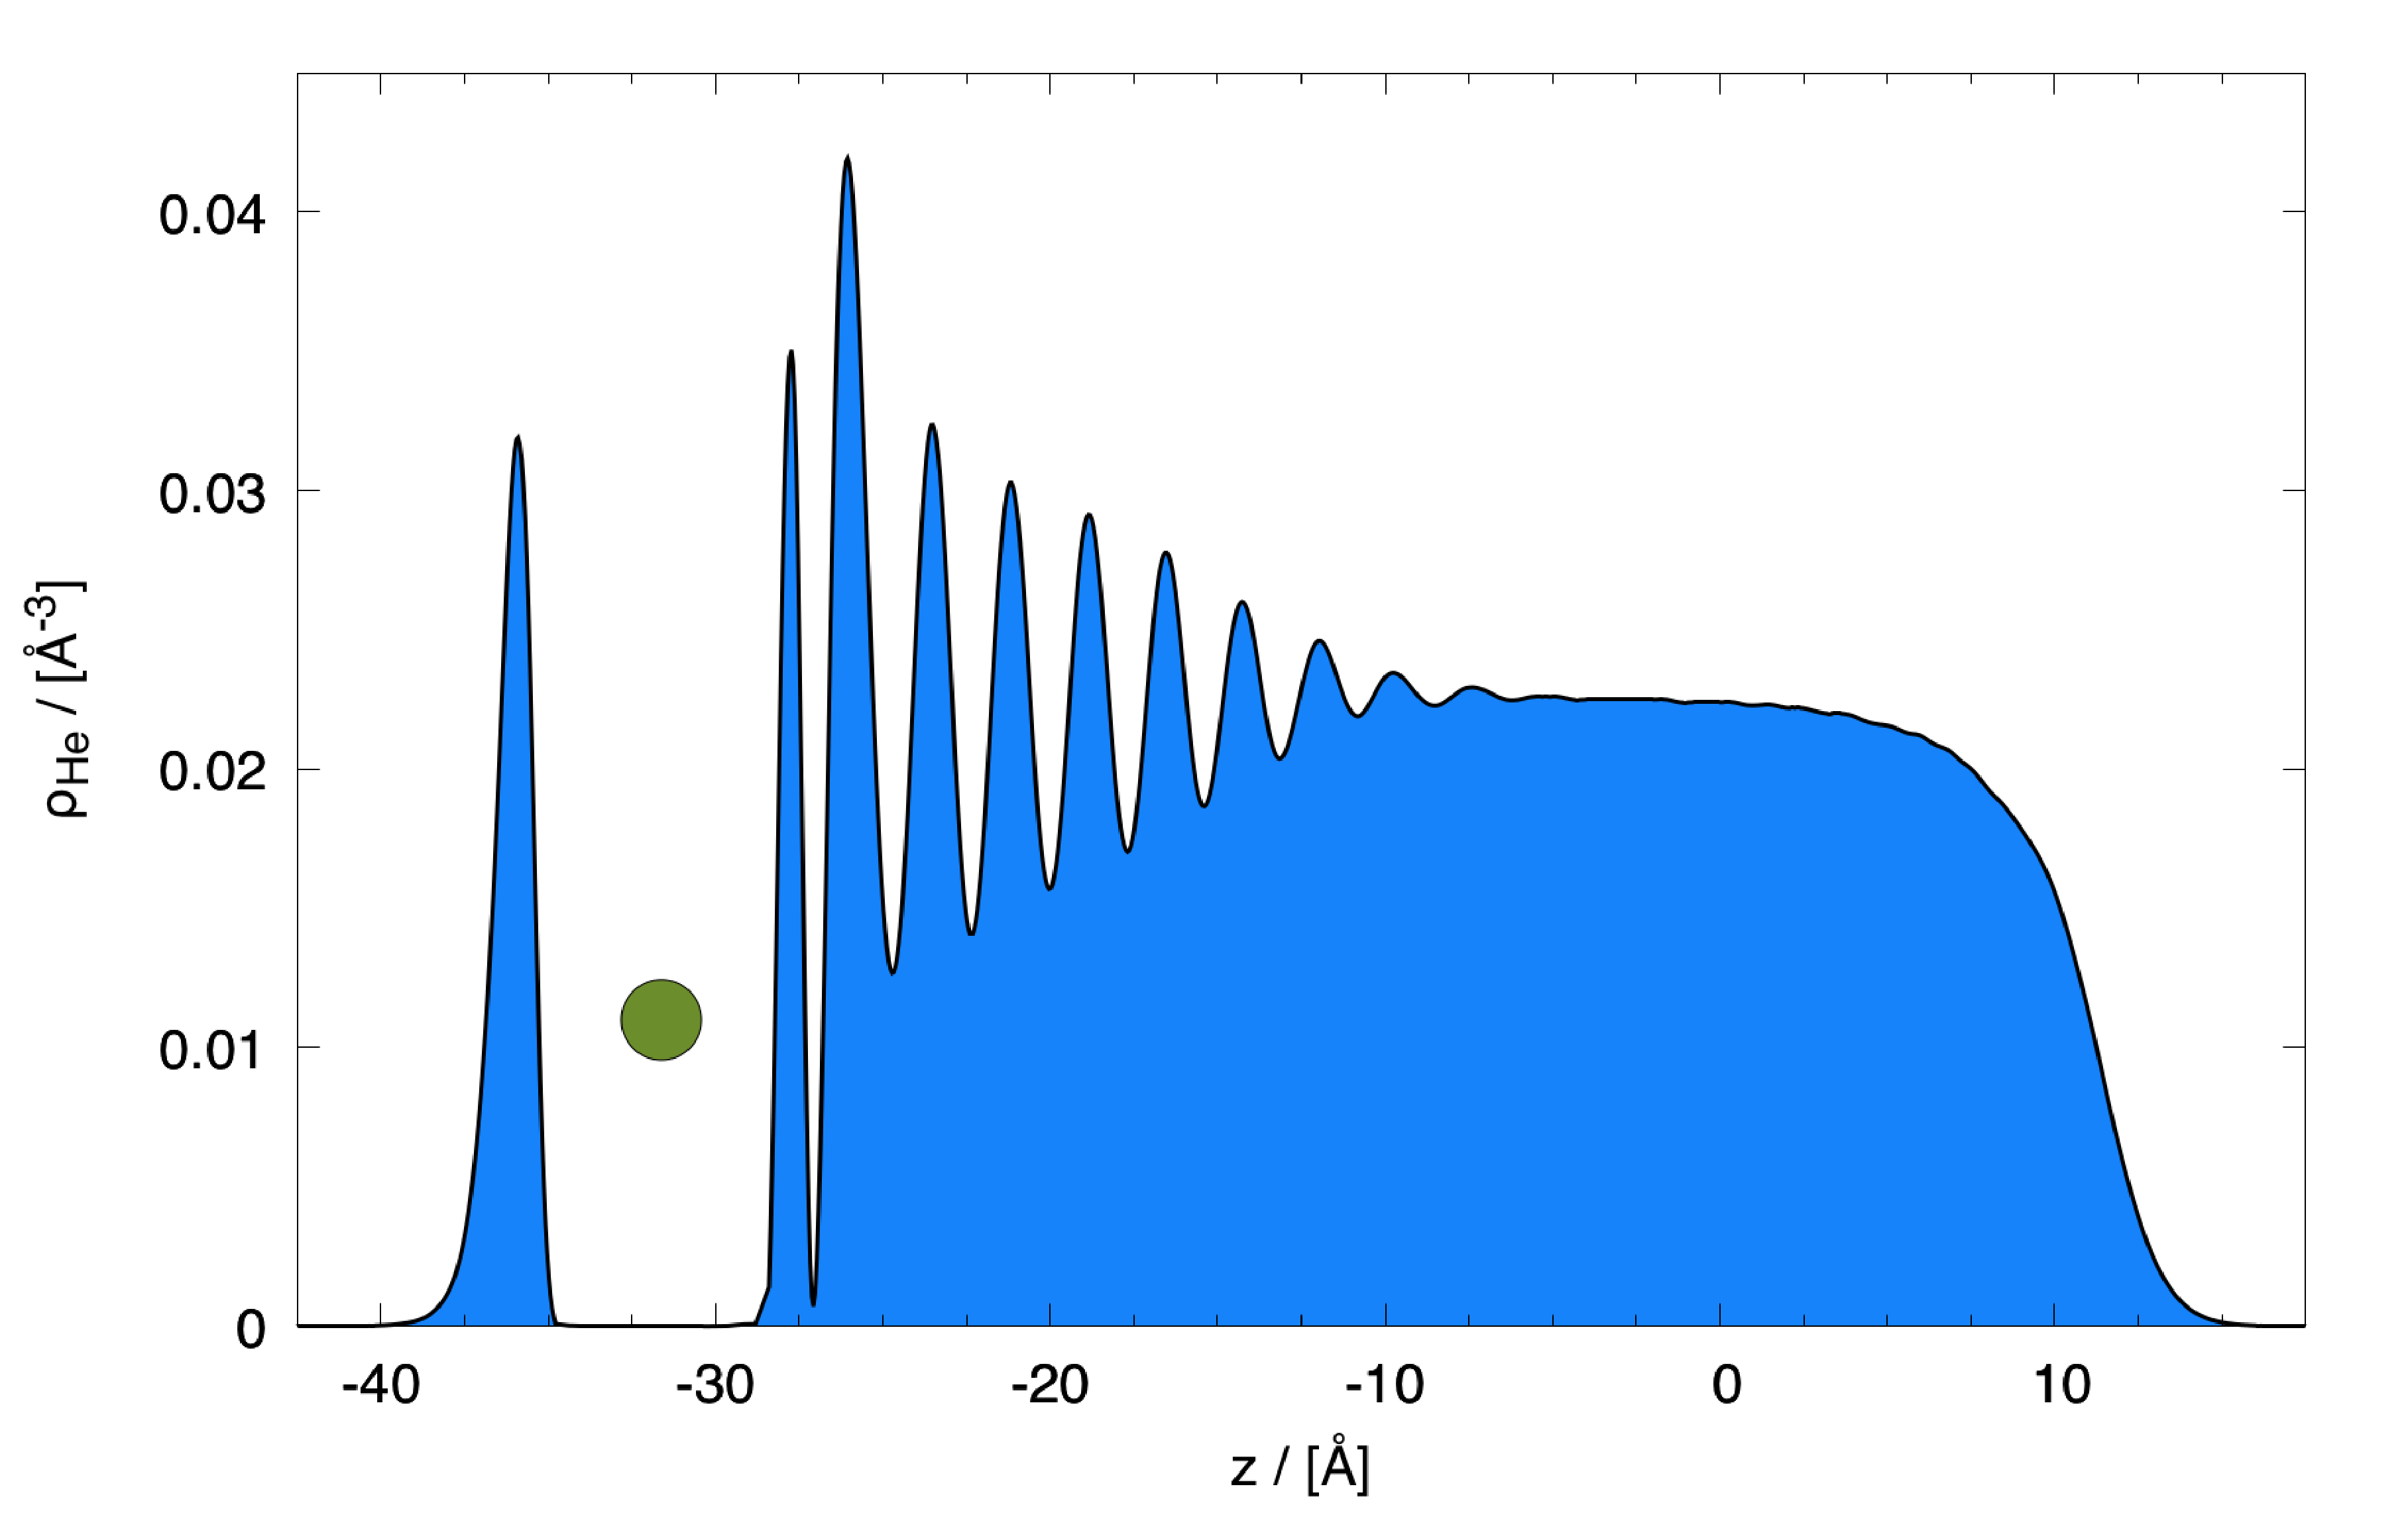
\includegraphics[width=1.0\linewidth]{fig4}
	\caption{Photoelectron energies as a function of pump-probe delay (filled circles) recorded at laser wavelengths $\lambda=794$~nm (5p$\Pi_{1/2}$) (a), $\lambda=773$~nm (5p$\Sigma_{1/2}$), and $\lambda=776$~nm (5p$\Pi_{3/2}$) (b). Open circles indicate the electron energies measured for atomic Rb background signal.}
	\label{fig:eK}
\end{figure}
\subsection{Photoelectron imaging}
\label{sec:PES}
The photoelectron spectra recorded at the three characteristic laser wavelengths $\lambda$ [Figure~\ref{fig:VMI} b)] exhibit pronounced peaks around the Rb 5p$_{1/2}$ and 5p$_{3/2}$ atomic binding energies, $E_{5p1/2}$ and $E_{5p3/2}$, respectively. Both the peak position and the peak width significantly vary with $\lambda$, as inferred from fits to the data with a Gaussian function, depicted as smooth lines. The resulting peak positions relative to $E_{5p1/2}$ and $E_{5p3/2}$ are plotted in Figure~\ref{fig:eK} a), b), respectively. Figure~\ref{fig:eK} c) shows the peak Gaussian widths $\sigma$. For reference, the open symbols represent the peak positions measured for the Rb atomic background. The scatter of data points around the literature value (grey horizontal line) indicates the level of precision of our measurements.

The excess energies for the 5p$\Sigma_{1/2}$ and 5p$\Pi_{3/2}$-states, $E_b - E_{5p1/2, \, 5p3/2}$ shown in Figure~\ref{fig:eK} b), exhibit a fast decay ($E^e_1$, $\tau^e_1$) above and a slow decay ($E^e_2$, $\tau^e_2$) below $E_{5p3/2}$ (horizontal line at $y=0$). Therefore, these data are fitted with a biexponential decay function
\begin{align} 
E^e(t)=E^e_1\cdot\mathrm{exp}(-\ln2\cdot t/\tau^e_1)+E^e_2\cdot\mathrm{exp}(-\ln2\cdot t/\tau^e_2)+E^e_{\infty}.\qquad
\label{Eel(t)}
\end{align}
Here, $E^e_\infty$ denotes the asymptotic energy value at long delay times. When exciting the 5p$\Pi_{1/2}$-state at $\lambda=794$~nm, the transient droplet correlated peak position remains constant within the experimental scatter. Therefore, merely the mean value $E^e_1$ is determined. The resulting energies and time constants are summarized in table~\ref{tab:FitParsEl}. The increasing peak widths in the cases of $\lambda=773$ and $776$~nm are fitted by the simple exponential function given by Eq.~(\ref{E(t)}). 

\begin{table*}[t]
	\begin{center}
		\begin{tabular}{|c c | c c | c c | c|}
			\hline
			$\lambda$\,[nm] & State & $E^e_1$\,[1/cm] & $\tau^e_1$\,[ps] & $E^e_2$\,[1/cm] & $\tau^e_2$\,[ps] & $E^e_\infty$\,[1/cm]\\  
			\hline\hline
			773 & $\Sigma_{1/2}/\Pi_{3/2}$ & 32(2) & 15(2) & 63(4) & 683(130) & -53(5) \\
			776 & $\Pi_{3/2}/\Sigma_{1/2}$ & 36(2) & 13(2) & 110(4) & 709(70) & -96(5) \\
			794 & $\Pi_{1/2}$ & 33(2) & - & - & - & - \\
			\hline
		\end{tabular}
		\caption{Time constants and energies inferred from fits of equation~(\ref{Eel(t)}) to the transient photoelectron energies (Figure~\ref{fig:eK}).}
		\label{tab:FitParsEl}
	\end{center}
\end{table*}
The fact that the droplet-related photoelectron energy $E^e_1$ for the $\Pi_{1/2}$-state is constant but shifted with respect to the atomic value indicates that most of the Rb atoms remain attached to the droplet surface upon electronic excitation, in accordance with previous studies~\cite{Auboeck:2008,TheisenJPCL:2011}. Thus, the slowly rising Rb$^+$-ion signal measured at that wavelength, indicative for excited Rb desorption, reflects only a small fraction of Rb atoms, most of which actually remain bound to the droplets. The measured up-shift of electron energy of $E^e_1=33(2)$~cm$^{-1}$ is attributed to a lowering of the ionization threshold induced by the He environment. This value is in reasonable agreement with previous measurements, where the ionization threshold was found to be lowered by $50(10)$~cm$^{-1}$ at comparable conditions~\cite{TheisenJPCL:2011}. 

The similar dynamics of electron energies and ion yields for the $\Sigma_{1/2}$ and $\Pi_{3/2}$-states, a biexponential evolution with a fast component (tens of ps) and a slow component (hundreds of ps), are taken as a confirmation that two distinct relaxation processes occur simultaneously. The fast process -- prompt desorption of excited Rb off the He droplet -- is associated mainly with the $\Sigma_{1/2}$-component of the excited state, whereas the $\Pi_{3/2}$-component undergoes slow relaxation. The latter will be discussed in the following sections. Deviations of the time constants $\tau^i_1$ vs. $\tau_1^e$, and $\tau^i_2$ vs. $\tau_2^e$, are mainly due to the different nature of the observables. Both ion yields and speeds are affected by the dynamics occurring \textit{after} the probe-ionization, whereas electron spectra probe the electronic state (affected by the He configuration around the Rb) \textit{at the moment} of ionization. In particular, ion signals provide information only about that fraction of ions that eventually detach from the He droplets, whereas electron signals are measured for all photoionization events, including those where the ion falls back into the droplet; in this respect the electron spectra are the better probes of the full dynamics, with the restriction that we cannot distinguish between the final products (Rb, RbHe, and Rb attached to a He droplet).

%Reasons for an imperfect separation of the Sigma(=fast Rb) and Pi_3/2(=slow RbHe) signals are, aside from the broad laser spectrum/overlapping absorption bands: i) a possible contribution to impulsive desorption by some Rb atoms in the Pi_3/2-state which do not form RbHe prior to desorption – this adds “fast” Rb-signal at the Pi_3/2-excitation at 776nm; iii) a possible contribution of “slow” Rb^+ signal at 776nm due to RbHe-dissociation upon relaxation – we suppose that in the spin-flip reaction some RbHe may end up above the dissociation threshold.

We mention that at $\lambda=776$\,nm ($\Pi_{3/2}$-state), an extended low intensity distribution is present in the spectrum of Figure~\ref{fig:VMI} b) at higher electron binding energies $\geq 21,500~$cm$^{-1}$ (lower electron kinetic energies). We attribute this component to elastic scattering of photoelectrons with He atoms as they propagate through the He droplet. Low-energy features in photoelectron spectra due to electron-He scattering have been observed before, in particular when using one-photon ionization~\cite{Loginov:2005,Peterka:2006,Wang:2008,Buchta:2013}. The fact that this feature is most pronounced for the $\Pi_{3/2}$-excitation may be related to the more abundant formation of RbHe exciplexes which enhances the electron-He scattering probability.

%RbHeN
%773nm: beta_2=0.20(5), beta_4=-0.07(5)
%776nm: beta_2=0.01(5), beta_4=-0.11(5)
%794nm: beta_2=0.31(5), beta_4=-0.04(5)

%Rb effusive
%776nm: beta_2=0.35(5), beta_4=-0.16(5)
%794nm: beta_2=0.29(5), beta_4=-0.10(5)

\begin{figure}[!]
	\centering
	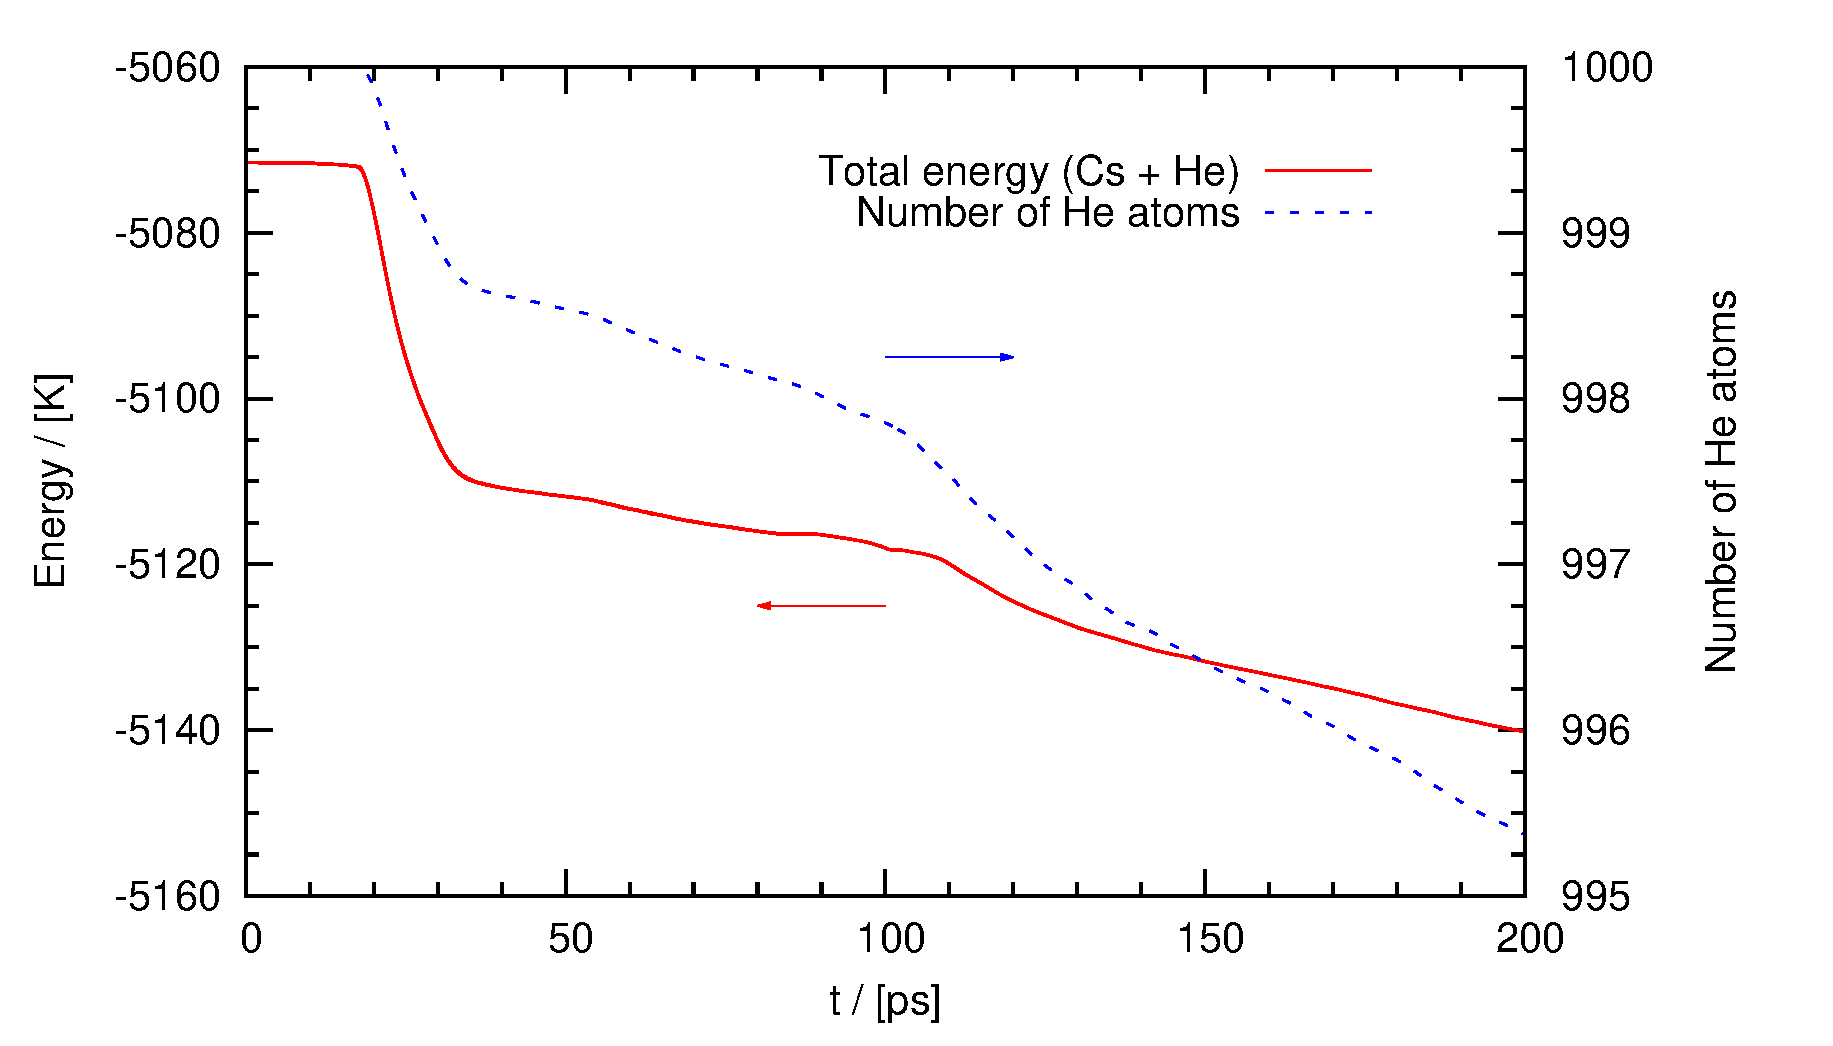
\includegraphics[width=0.9\linewidth,clip]{fig5}\caption{Snapshots of the He density during the evolution of the excited RbHe$_{1000}$ complex for $\eta=15$\%, $\Delta t=60$ps. The green dot represents the Rb atom excited into the 5p$\Pi_{3/2}$-state; the magenta dot is the Rb atom after suddenly relaxing to the 5p$\Pi_{1/2}$-state.}
	\label{fig:snapshots}
\end{figure}
%%%%%%%%%%%%%%%%%%%%%%%%%%%%%%%%%%%%%%%%%%%%%%%%%%%%%%%%%%%%
\section{TD-DFT dynamics simulation}
Time-dependent density functional theory (TD-DFT) simulations are carried out as thoroughly described in Refs.~\cite{Mateo:2013,Ancilotto:2017}. Starting with the Rb-droplet equilibrium configuration, the dynamics is initiated by a ``vertical DFT transition'' into the excited state. This is realized by suddenly switching from the potential energy surface of the Rb-He droplet ground state to that of the Rb-He excited state. The subsequent evolution of the system can be followed in real-time, as illustrated by the series of snapshots of the He density distribution (red area) and the position of the Rb atom (green and magenta dots) in Figure~\ref{fig:snapshots}. Here, excitation of the 5p$\Pi_{3/2}$-state at $t=0$ is followed by relaxation to the 5p$\Pi_{1/2}$-state at $t=60$~ps. 

%{\bf WE COULD GIVE  DETAILS ON THE DYNAMICS, BUT I'VE WRITTEN THE EQUATIONS SO MANY TIMES THAT I DON'T KNOW HOW TO PRESENT THEM A BIT DIFFERENTLY}

\begin{figure}[!]
	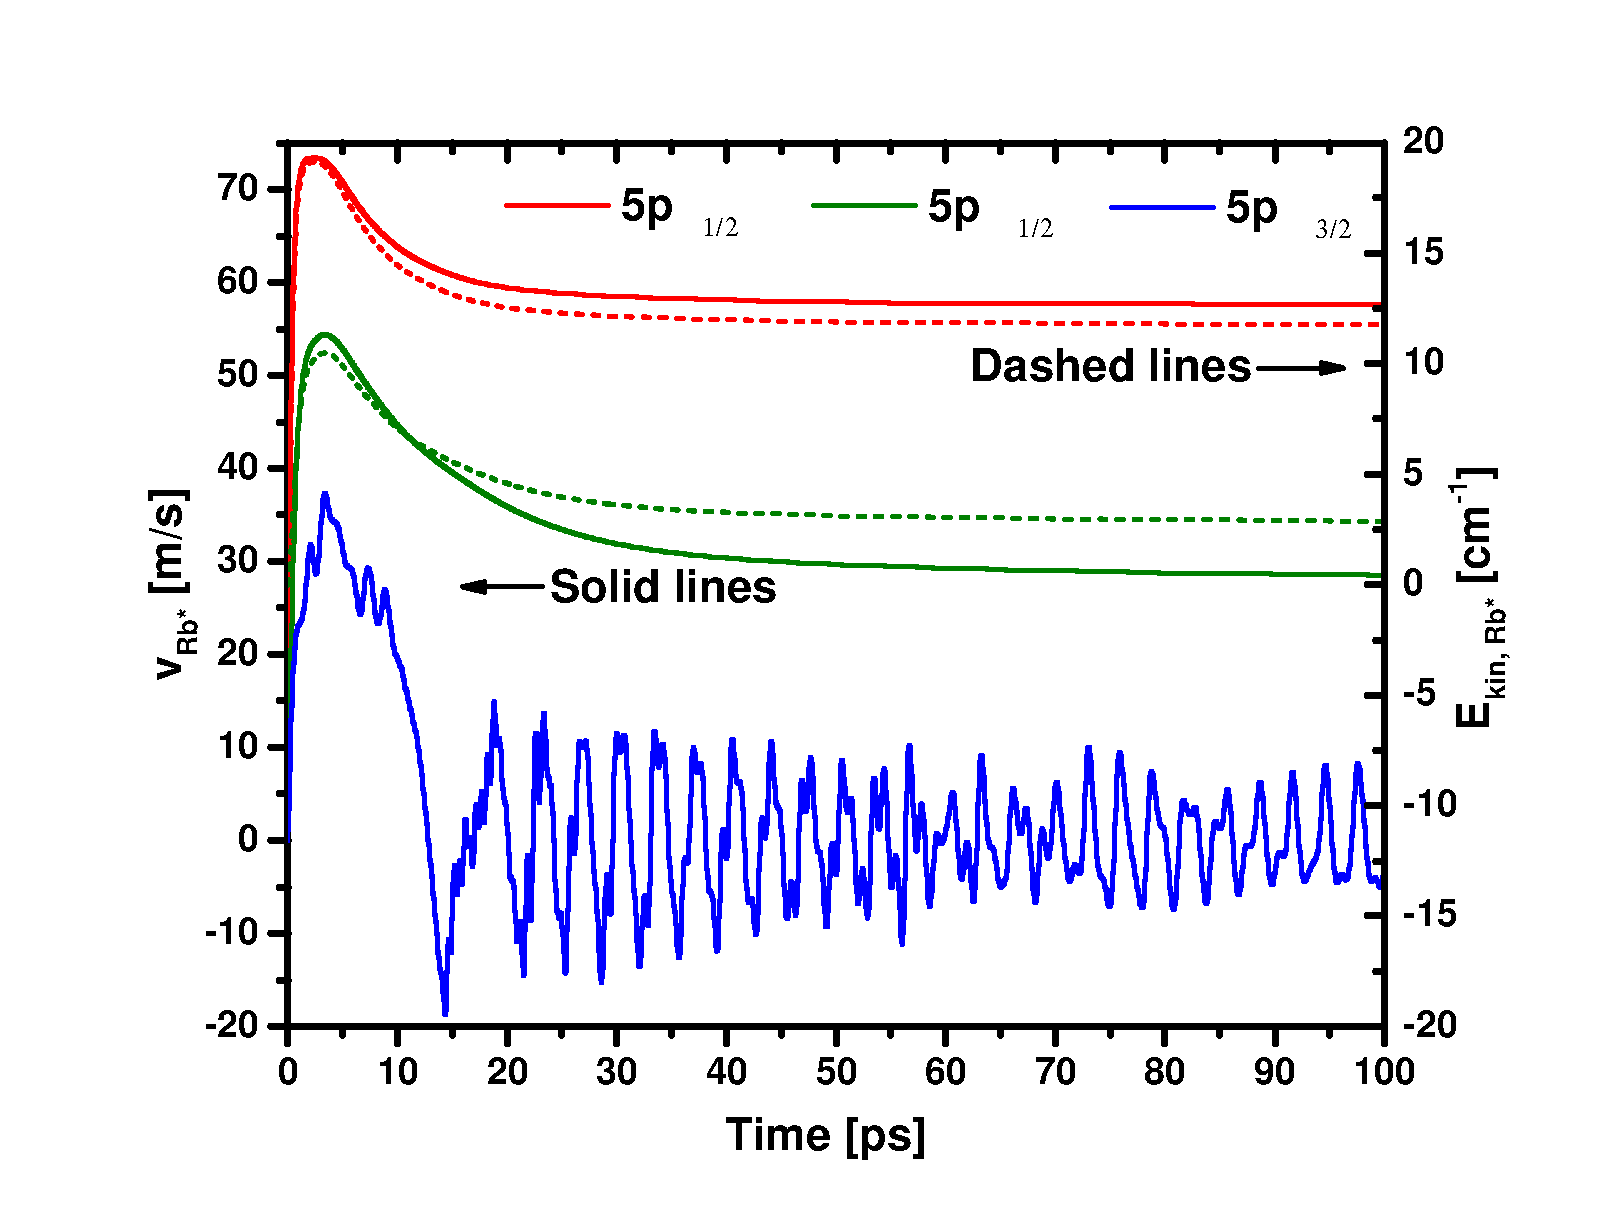
\includegraphics[width=1.0\linewidth,clip=true]{fig6}
	\caption{\label{fig:simvel} 
		Velocity (solid lines, left scale) and kinetic energy (dashed lines, right scale) of the Rb atom excited to the 5p-state as a function of time. The kinetic energy of the 5p$\Pi_{3/2}$-state is not given as this state remains bound to the droplet.}
\end{figure}
%%%%%%%%%%%%%%%%%%%%%%%%%%%%%%%%%%%%%%%%%%%%%%%%%%
\subsection{Direct ejection of bare Rb atoms from the $^2\Sigma_{1/2}$ and $^2\Pi_{1/2}$-states}
From these data we now infer the relevant quantities to compare with the experimental results, such as the kinetic energy of the Rb atom relative to the droplet, the occurrence of He density attached to Rb which we identify with the formation of an exciplex, and the transient interaction energy of the neutral and ionized Rb atom with the surrounding He. The latter is related to the kinetic energy of a photoelectron created in a time-delayed photoionization process. 

Figure~\ref{fig:simvel} collects our results for the dynamics of the Rb atom excited to the droplet-perturbed states correlating to the atomic 5p-state. For the $\Sigma_{1/2}$ and $\Pi_{1/2}$-states, the velocities (dashed lines) and kinetic energies (solid lines) feature a rapid increase to reach a maximum at time $t=2$-$5$~ps after excitation, followed by a drop due to long-range attractive forces acting on the desorbing Rb atom. The asymptotic values are reached for $t>50~$ps. When exciting the $\Pi_{3/2}$-state, the Rb-velocity features a damped oscillation around zero indicating that the Rb atom remains bound to the He droplet surface. The following conclusions can be drawn from these results: 

(i) Rb excited to the 5p$\Sigma_{1/2}$-state detaches from the droplet reaching an asymptotic kinetic energy of 13~cm$^{-1}$. This value deviates from the experimental one (8.0~cm$^{-1}$) due to contributions of $\Pi_{3/2}$-excitation to the experimental signal. Despite of the shallow local minima in the corresponding Rb-He droplet potential surface [\ref{fig:pots} c)], no binding of He density to the departing Rb atom occurs. This finding is in accordance with experiments~\cite{Bruehl:2001,Droppelmann:2004,Fechner:2012}, where mostly free Rb atoms were detected following excitation at wavelengths $\lambda<774$~nm. 

(ii) Rb excited to the 5p$\Pi_{1/2}$-state also detaches from the He droplet, but the asymptotic kinetic energy is much lower, 2.8~cm$^{-1}$. 
%This is due to the weaker repulsion compared to the 5p$\Sigma_{1/2}$-state. 
This value again deviates from the experimental one (5.1~cm$^{-1}$), but the trend that desorption of the less repulsive $\Pi_{1/2}$-state yields a lower energy than for the $\Sigma_{1/2}$-state is well reproduced. The potential well at short distance $\sim 3~$\AA{} would in principle support a stable RbHe exiplex. However, at the low temperature of the He droplet, exciplex formation is hindered by a potential barrier located at $\sim 5$~\AA{}, between the well and the range where the 5p$\Pi_{1/2}$-state is populated by excitation from the 5s$\Sigma_{1/2}$-ground state (7~\AA{})~\cite{Reho2:2000,Bruehl:2001,Hirano:2003}.

We recall that in previous experiments using narrow-band excitation of the low energy edge of the $\Pi_{1/2}$-resonance, it was observed that Rb and Cs dopants remained attached to the He droplet surface~\cite{Auboeck:2008}. However, our simulations correspond to the excitation at the peak of the resonance, where free Rb atoms are also observed in the experiment. Thus, our simulations are not in conflict with the experimental findings. Note that Quantum Monte Carlo (QMC) calculations carried out for this state~\cite{Leino:2008} yielded a weakly bound Rb in a shallow dimple. Had we carried out a {\it static} DFT relaxation, we would also have found a bound structure, due to the shallow minimum on the Rb-He droplet potential surface. However, in the dynamical TD-DFT simulation this minimum is too shallow to retain the departing Rb atom.

(iii) In our simulation we find that Rb excited to the 5p$\Pi_{3/2}$-state remains bound to the He droplet surface where it forms a RbHe exciplex. Figure~\ref{fig:pots} shows two deep barrierless potential wells at a Rb-He distance of about 3~\AA{}. In the course of the dynamics, the Rb atom is drawn to the well close to the droplet surface, develops a RbHe exciplex that remains bound to it, and oscillates around an equilibrium position of $\sim 3$~\AA{} above the static equilibrium position at the dimple as shown in Figure~\ref{fig:simvel}. This result is in full agreement with static QMC calculations by Leino et al.~\cite{Leino:2011}. Note that our simulations do not provide any indication that the vibrational motion of the RbHe exciplex structure leads to its desorption from the He droplet. 
	
\begin{figure}[!]
	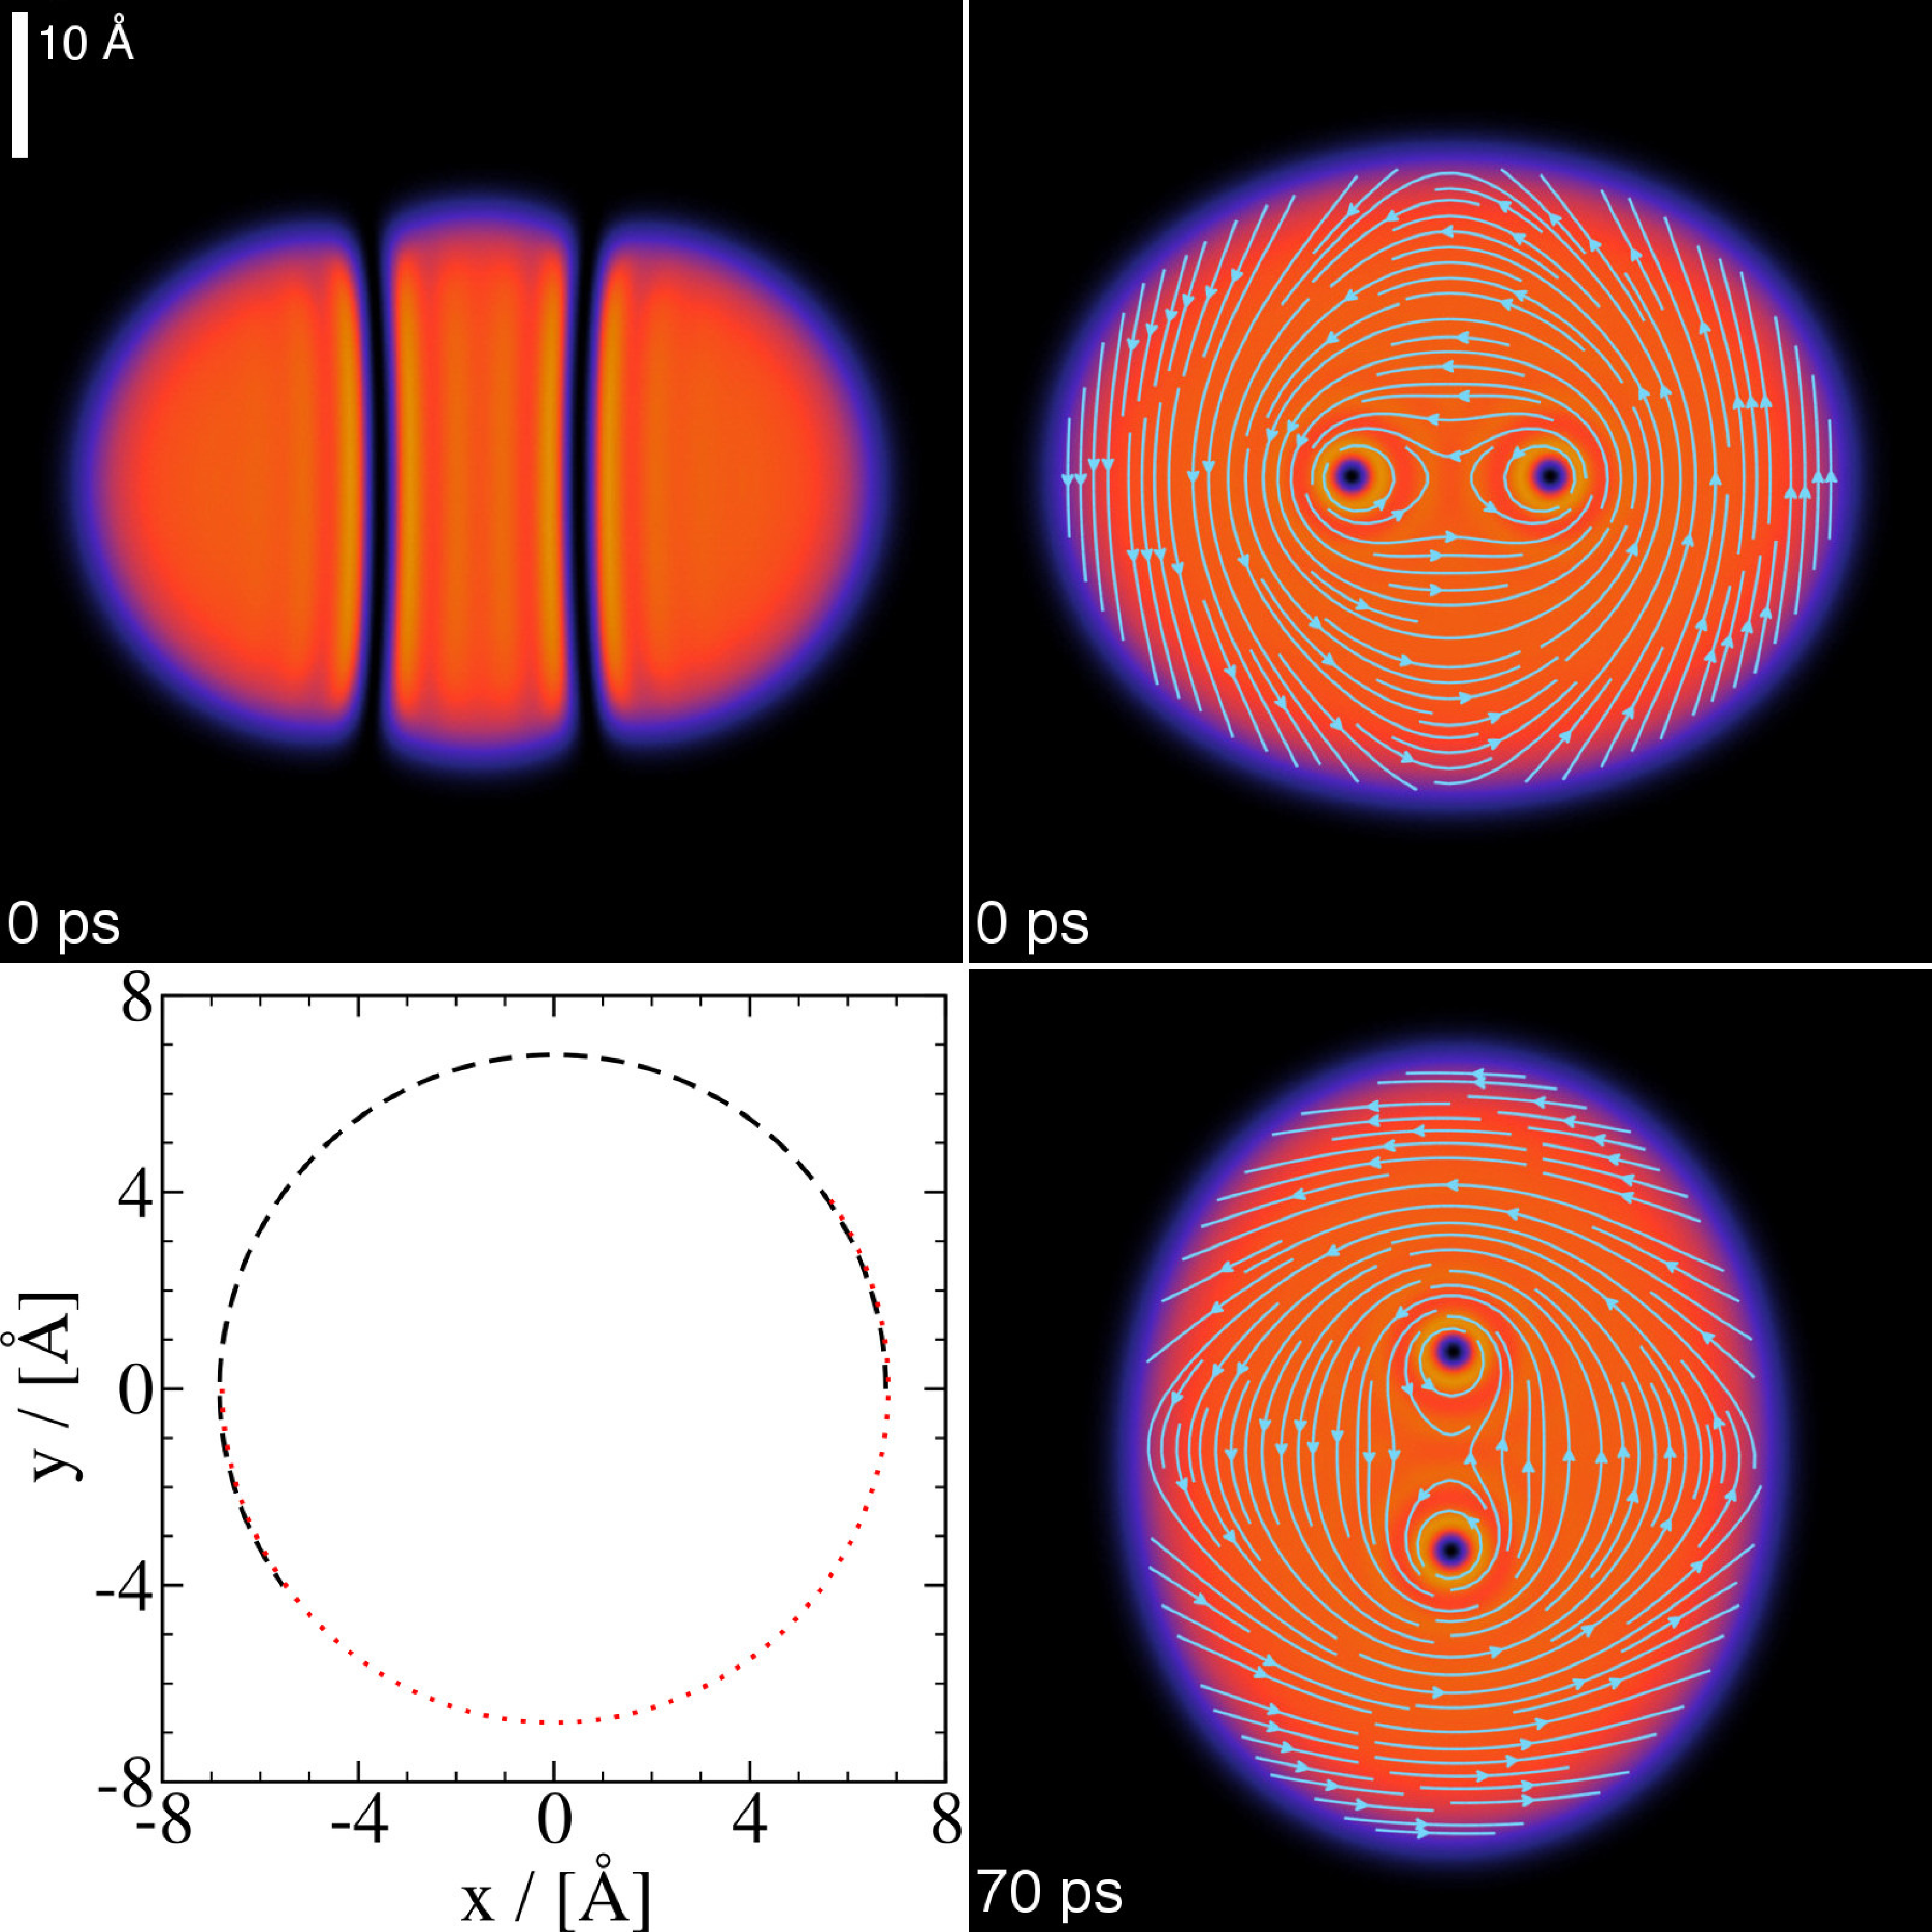
\includegraphics[width=1.0\linewidth,clip=true]{fig7}
	\caption{\label{fig:inclusion} Simulated time evolution of the integrated He density within an inclusion volume of radius $r_{\mathrm incl}=5.7~$\AA{} around the Rb atom excited to the 5p$\Pi_{3/2}$-state.}
\end{figure}
The dynamics of the exciplex formation process can be quantitatively represented by integrating over the He density within a spherical inclusion volume with radius $r_\mathrm{incl}$ around Rb. The result is shown in Figure~\ref{fig:inclusion}. Thus, for $r_\mathrm{incl}=5.7~$\AA{}, which contains the entire localized He density at the Rb atom without including He density of the remaining droplet, we find a rise to 75~\% of the final value at $t=20$~ps. For $t>60$~ps the He number density stabilizes close to 1, indicating the full evolution of a RbHe exciplex containing 1 He atom. This result is in good agreement with the formation time estimated using the tunneling model by Reho et al.~\cite{Reho2:2000} using model parameters inferred from the previous fs-ps pump-probe measurements ($42$~ps)~\cite{Giese:2012}.
%, where an increasing [RbHe]$^+$ signal was observed that reached its maximum at a delay time of about $20$~ps~\cite{Droppelmann:2004,Mudrich:2008}.

The finding that the RbHe exciplex remains attached to the He droplet is in apparent contradiction to experiments where the ejection of free Rb and RbHe was clearly observed~\cite{Bruehl:2001,Droppelmann:2004,Fechner:2012}. Therefore, an additional mechanism must be active that induces the desorption of the RbHe molecule off the He droplet surface.

\begin{table}[!]
	%\small
	\centering
	\vspace{0.1 cm}
	\begin{tabular}{ccc}
		\hline 
		$\eta$ (\%) &  $v_\infty$(m/s) & Kin. energy (cm$^{-1}$) \\ 
		\hline
		5   & bound & -- \\
		10  & 13.4  & 0.64\\ 
		12.5 & 43.0 & 6.6 \\
		15  & 62.4 & 13.9 \\ 
		20  & 80.4& 23.0 \\ 
		\hline 
	\end{tabular} 
	\caption{\label{tab1} 
	Asymptotic velocity and kinetic energy of the ejected RbHe exciplex for various values of the fraction $\eta$ of the 5p$\Pi_{3/2,\, 1/2}$-energy spacing of 165~cm$^{-1}$, which is converted into kinetic energy of Rb by relaxation from the 5p$\Pi_{3/2}$ into the 5p$\Pi_{1/2}$-state. The calculations are carried out at a delay time $\Delta t=60$~ps between photo-excitation and non-radiative de-excitation of the Rb atom.
} 
\end{table} 

\subsection{RbHe exciplex formation around the 5p$^2\Pi_{1/2}$-state: non-radiative relaxation from the 5p$^2\Pi_{3/2}$-state}
In the gas phase, a RbHe exciplex can form in the 5p$\Pi_{1/2}$-state if enough kinetic energy is provided by collisions such that the Rb can overcome the potential barrier~\cite{Hirano:2003}. Alternatively, collisions of a RbHe formed in the 5p$\Pi_{3/2}$-state with another atom or complex might induce relaxation into a RbHe electronic state correlating to the Rb 5p$_{1/2}$-state. In this case the barrier is circumvented by the relaxation process, as the potential wells for the two states $\Pi_{3/2}$ and $\Pi_{1/2}$ are at similar Rb-He distances. In the condensed (droplet) phase at 0.4~K temperature, none of these mechanisms are active to explain the formation of RbHe 5p$^2\Pi_{1/2}$ exciplexes and their potential ejection.    

However, Figure~\ref{fig:pots} a) indicates another possible mechanism: Non-radiative de-excitation from the 5p$\Pi_{3/2}$ to the 5p$\Pi_{1/2}$-state accompanied by transfer of energy into the relative motion of the Rb atom away from the He droplet. Notice from the figure that the minimum of the 5p$\Pi_{3/2}$-potential is at $\sim 12683$~cm$^{-1}$, and that of the 5p$\Pi_{1/2}$-potential is at $\sim 12518$~cm$^{-1}$; the value of this potential at the barrier is $12611$~cm$^{-1}$. Thus, non-radiative de-excitation of the Rb atom may add to its original kinetic energy a fraction of this 165~cm$^{-1}$ difference energy. Consequently, the RbHe exciplex will be ejected in the 5p$\Pi_{1/2}$-state, and not in the 5p$\Pi_{3/2}$-state that was originally photo-excited. Non-radiative electronic relaxation induced by the He droplet has been observed for a number of metal atoms~\cite{Loginov:2007,Fechner:2012,Kautsch:2013,Koch:2014,Lindebner:2014,Loginov:2014,Loginov:2015}. In particular, previous measurements of the dispersed fluorescence emitted upon excitation of Rb into the 5p$\Pi_{3/2}$-state of the Rb-He droplet complex have evidenced large populations of free Rb atoms in the 5p$\Pi_{1/2}$-state~\cite{Bruehl:2001}. Efficient spin-relaxation of 5p$\Pi_{3/2}$-excited Rb atoms can be rationalized by the large cross section for mixing of fine structure states in collisions of alkali metal atoms with He~\cite{Krause:1975}. For low-temperature Rb-He collisions, the fine structure relaxation rate was found to be enhanced by the transient formation of a RbHe exciplex by orders of magnitude compared to binary Rb-He collisions~\cite{Hirano:2003}.

Here, we explore this scenario within TD-DFT. Starting from Rb in the 5p$\Pi_{3/2}$-state, we induce a ``vertical DFT transition'' by suddenly switching potential energy surfaces from 5p$\Pi_{3/2}$ to 5p$\Pi_{1/2}$, imparting to the Rb a kinetic energy corresponding to a fraction $\eta$ of the available non-radiative de-excitation energy. The time $\Delta t$ elapsing between the vertical excitation and de-excitation has to be chosen as well; this time influences the degree of RbHe 5p$\Pi_{3/2}$ exciplex formation which, as we have seen, may require some tens of ps. The actual value of these inputs cannot be determined by the model itself.

\begin{figure}[!]
	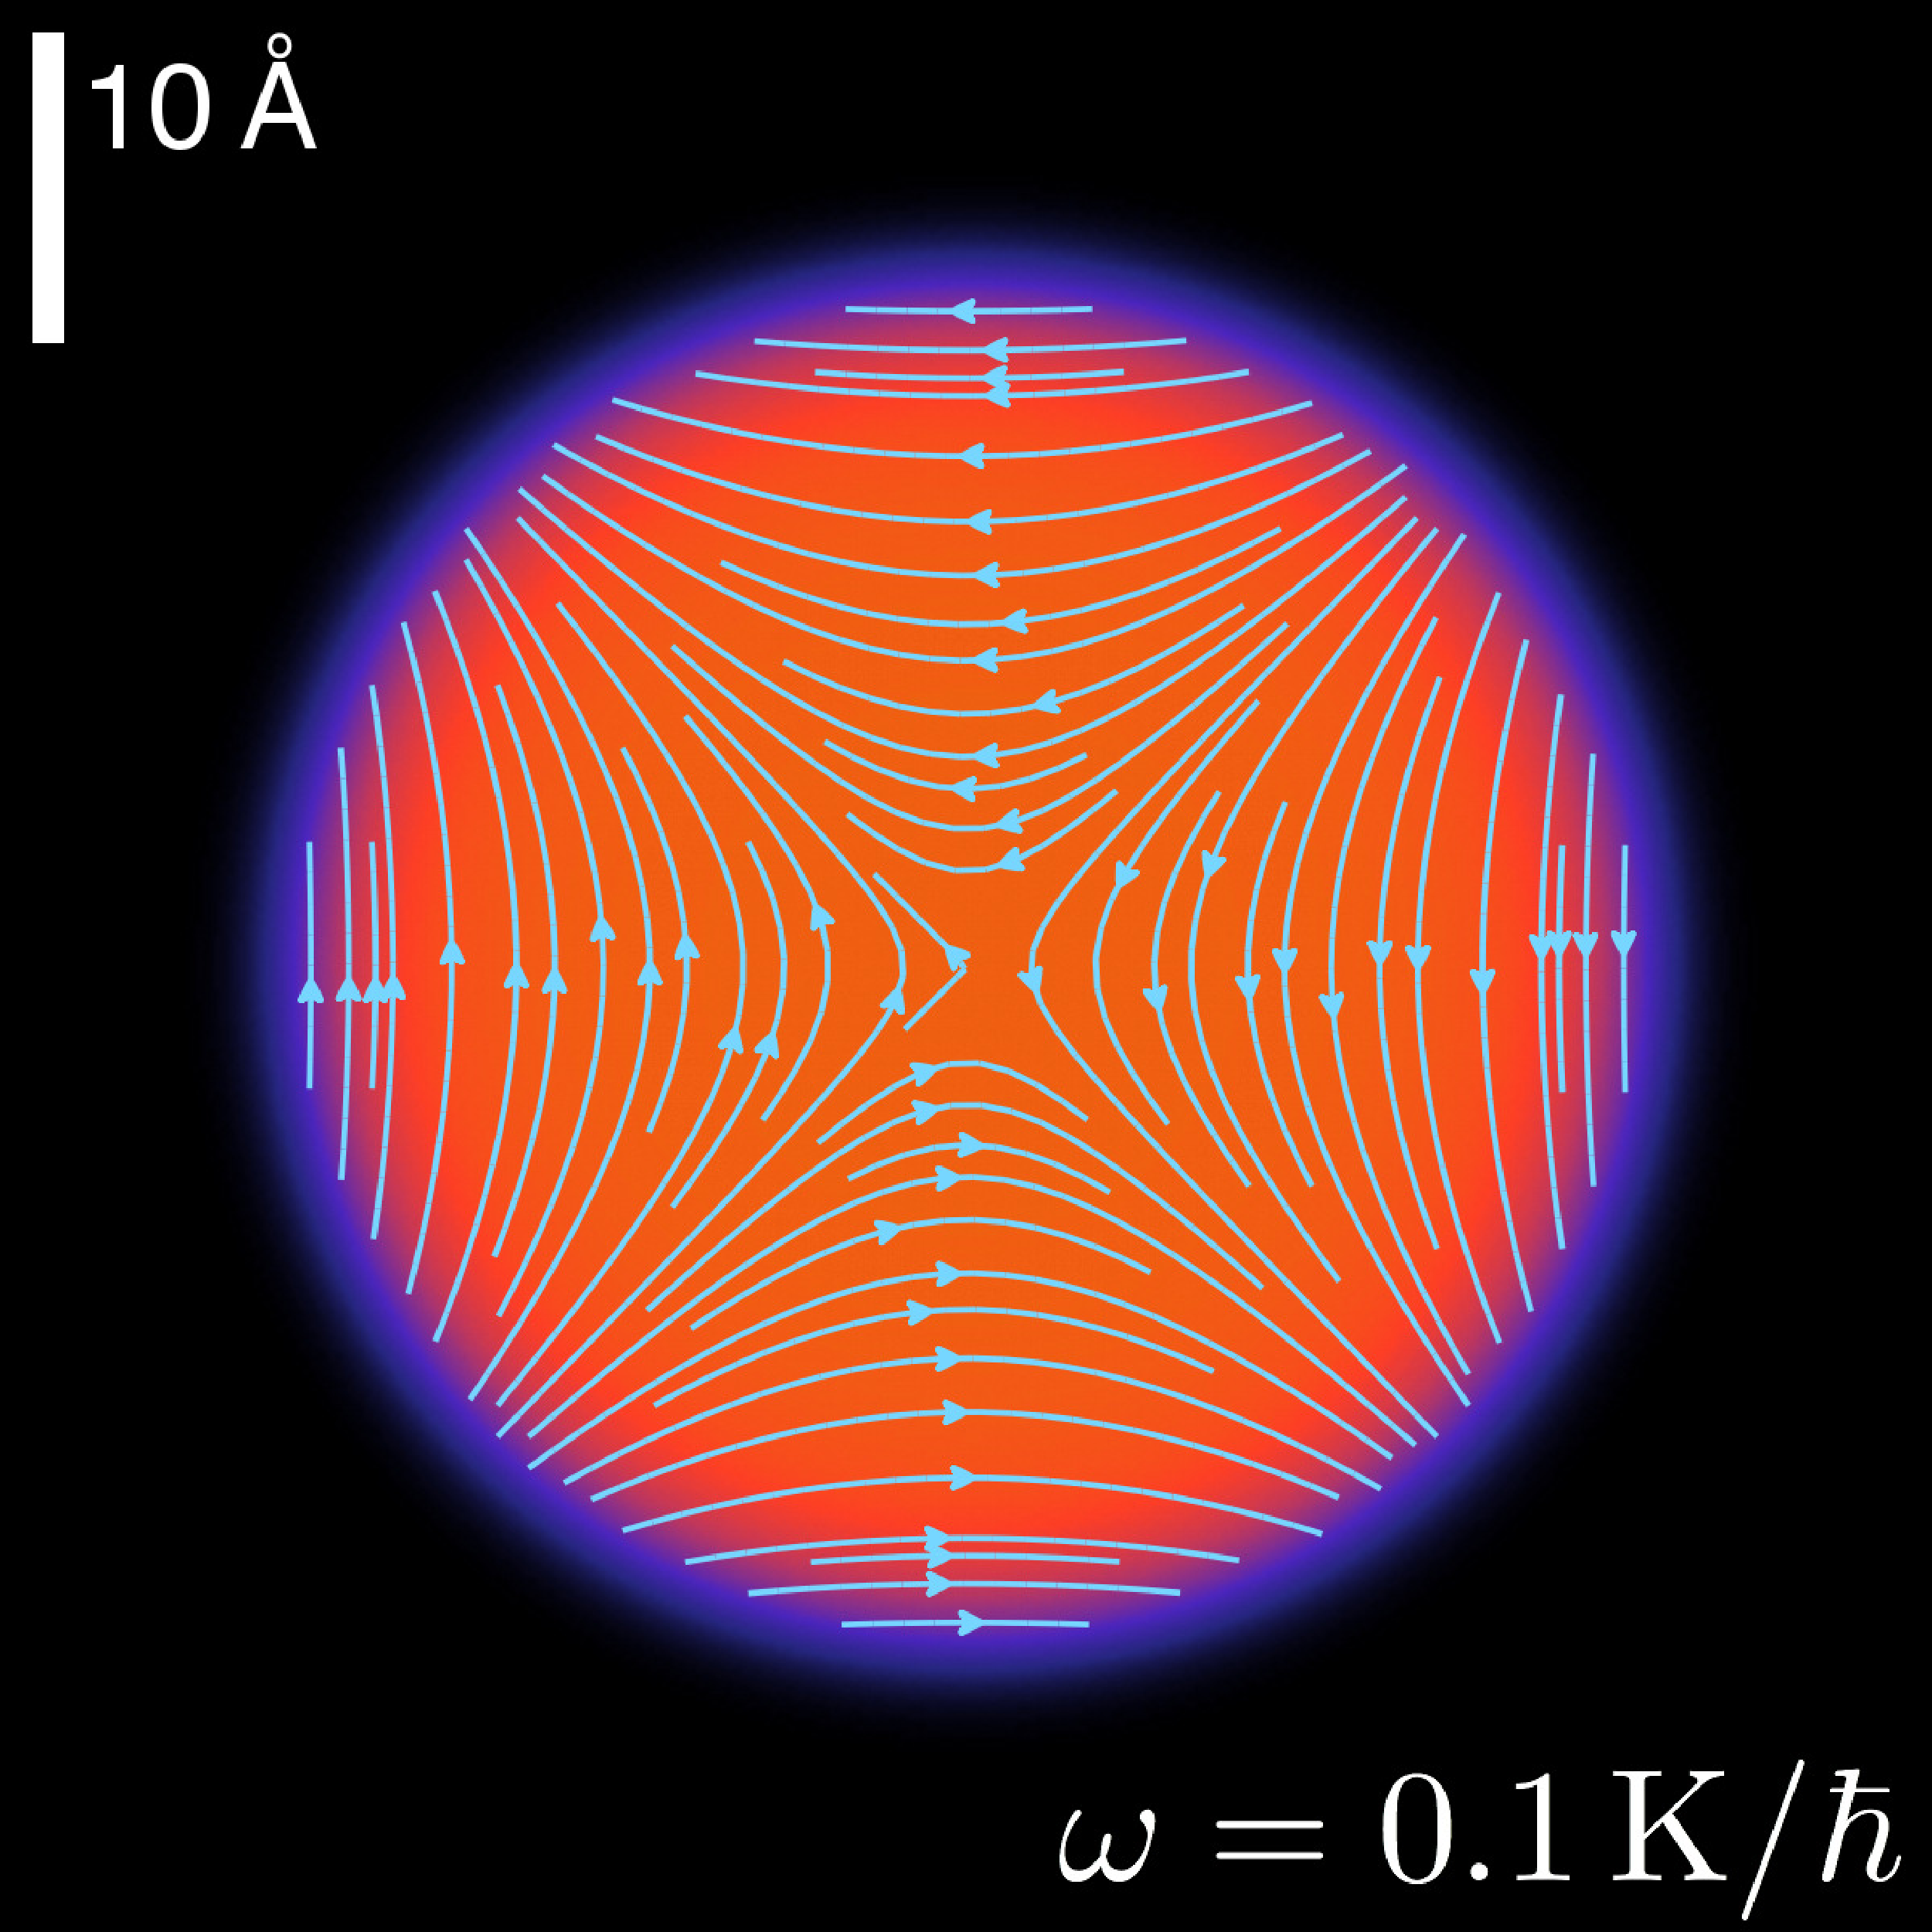
\includegraphics[width=1.0\linewidth,clip=true]{fig8}
	\caption{\label{fig:speed_eta} Velocity of the excited Rb atom with attached He density as a function of time after 5p$\Pi_{3/2} \rightarrow$5p$\Pi_{1/2}$ relaxation at $\Delta t=60$~ps for various values of the energy conversion factor $\eta$.}
\end{figure}
In the following, we present results obtained from simulations using as input parameters the delay before relaxation $\Delta t=60$~ps, and several values of $\eta$. As shown in Figure~\ref{fig:simvel} (see also the bottom left panel of Figure~\ref{fig:snapshots}), this --arbitrary--  time is sufficient to allow for a full development of the 5p$\Pi_{3/2}$ RbHe exciplex and to bring it to a rather stationary configuration. Figure~\ref{fig:snapshots} shows snapshots of the evolution following the 5s$\Sigma_{1/2}\rightarrow$5p$\Pi_{3/2}\rightarrow$5p$\Pi_{1/2}$ process for $\eta=15$\%, $\Delta t=60$~ps. Thus, upon sudden relaxation to the 5p$\Pi_{1/2}$-state, the RbHe structure promptly detaches from the remaining He droplet. The velocity of the Rb atom as a function of time is depicted in Figure~\ref{fig:speed_eta} for this and other values of $\eta$. Clearly, as the fraction of relaxation energy converted to Rb kinetic energy is increased from 10\,\% to 15\,\%, the initial speed, and even more so, the asymptotic value for long evolution times rises significantly. Table~\ref{tab1} collects the results obtained for various values of $\eta$. It can be seen that a fairly small $\eta\geq 10\,$\% is enough to induce the ejection of the RbHe complex. For a value $\eta = 12.5\,$\%, the asymptotic value of the RbHe velocity matches best the experimental one measured for maximum 5p$\Pi_{3/2}$-excitation at $\lambda = 776~$nm. 

When assuming that the relaxation-induced RbHe desorption proceeds as an impulsive dissociation reaction, the conversion factor $\eta$ can be related to an effective mass of the He droplet, $m_{eff}$~\cite{Hernando:2012}. From $\eta = 12.5\,$\% we obtain $m_{eff}=12.7$~amu, which corresponds to about 3 He atoms effectively interacting with the excited RbHe. This value is significantly less than what was found for the prompt desorption of Rb and RbHe upon excitation of the Rb 6s and 6p-correlated states~\cite{Fechner:2012,Vangerow:2014}. This is no surprise, though, since the orbital overlap between the excited RbHe and the He droplet is smaller than for the higher excited and more extended 6s and 6p-states. Besides, the effective mass model is not strictly valid in the present situation, since it neglects the internal degrees of freedom of RbHe which is taken as one fixed subunit.

Now that we have established the RbHe formation and desorption mechanisms, we can take our comparative study one step further and compute from the simulation results the electron binding energies to compare with the experimental photoelectron spectra. For this, we evaluate the interaction energy of the excited Rb atom and of the Rb$^+$ ion with the droplet by calculating, respectively, 
%
\begin{equation}
U^*(t) = \int  \, d \mathbf{r} \, {\cal V}_\mathrm{\mathbf{He-Rb^*}} (|\mathbf{r} -  \mathbf{r}_\mathrm{\mathbf{Rb^*}}|) \, \rho(\mathbf{r},t)
\label{eq77}
\end{equation}
%
and  
%
\begin{equation}
U^+(t) = \int  d \mathbf{r}  \, {\cal V}_\mathrm{\mathbf{He-Rb^+}} (|\mathbf{r} -  \mathbf{r}_\mathrm{\mathbf{Rb^+}}|) \, \rho(\mathbf{r},t)
\label{eq779}.
\end{equation}
%
Here the He-Rb$^+$ pair potential ${\cal V}_\mathrm{\mathbf{He-Rb^+}}$ is taken from  Ref.~\cite{Leal:2014}. 

\begin{figure}[!]
	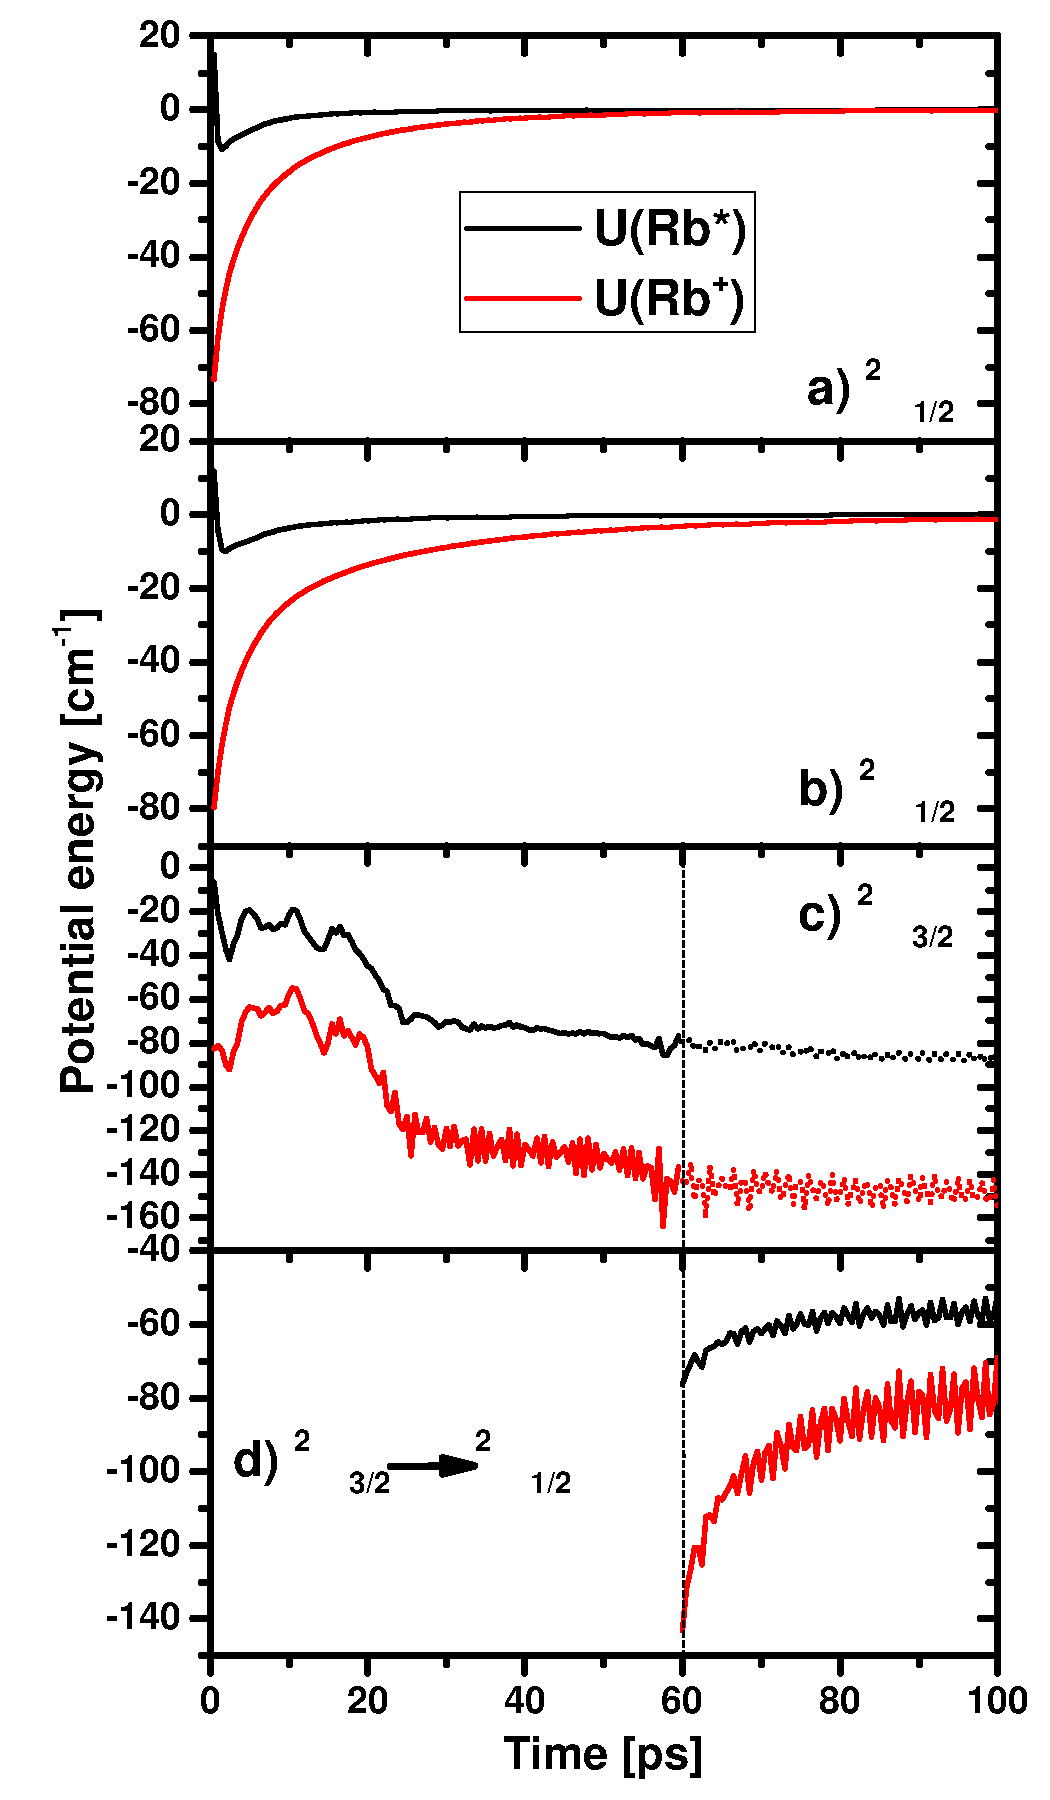
\includegraphics[width=1.0\linewidth,clip=true]{fig9}
	\caption{\label{fig:Ustar} Simulated energies of the Rb-atom excited into various states interacting with the surrounding He distribution (black lines), and of the Rb$^+$ ion for the same momentary geometry (red lines). In d), the excited state of Rb is suddenly switched from $\Pi_{3/2}$ to $\Pi_{1/2}$ to simulate the dynamics initiated by spin-relaxation.}
\end{figure}
The interaction energies $U^*(t)$ and $U^+(t)$ are shown in Figure~\ref{fig:Ustar} for Rb in the $\Sigma_{1/2}$-state in a), for the $\Pi_{1/2}$-state in b), and for the $\Pi_{3/2}$-state in c). Figure~\ref{fig:Ustar} d) shows the evolution following the sudden relaxation of Rb to the  $\Pi_{1/2}$-state at $t=60~$ps. The prompt desorption of Rb in the $\Sigma_{1/2}$ and $\Pi_{1/2}$-states is seen as a sudden drop of $U^*(t)$ near $t=0$ followed by a slow rise towards zero due to long-range van der Waals attraction as Rb departs from the He droplet. Due to the purely attractive interaction of the Rb$^+$ ion with the He droplet, $U^+(t)$ monotonically rises to zero. The exciplex formation dynamics in the $\Pi_{3/2}$-state is reflected by the irregular behavior of $U^*(t)$ and $U^+(t)$, eventually stabilizing at $t>60$~ps at negative values, \textit{i.\,e.} in a configuration where Rb is bound to the He droplet. Only when allowing for a sudden relaxation into the $\Pi_{1/2}$-state at $t=60~$ps, the RbHe exciplex receives a momentum ``kick'' and subsequently detaches from the He droplet, in spite of a rising $U^*(t)$. The asymptotic values of $U^*$ and  $U^+$ are then given by the binding energy of the free RbHe exciplex configuration. The fast oscillations at $t>65$~ps indicate that RbHe keeps vibrating as it is ejected.

\begin{figure}[!]
	\centering
	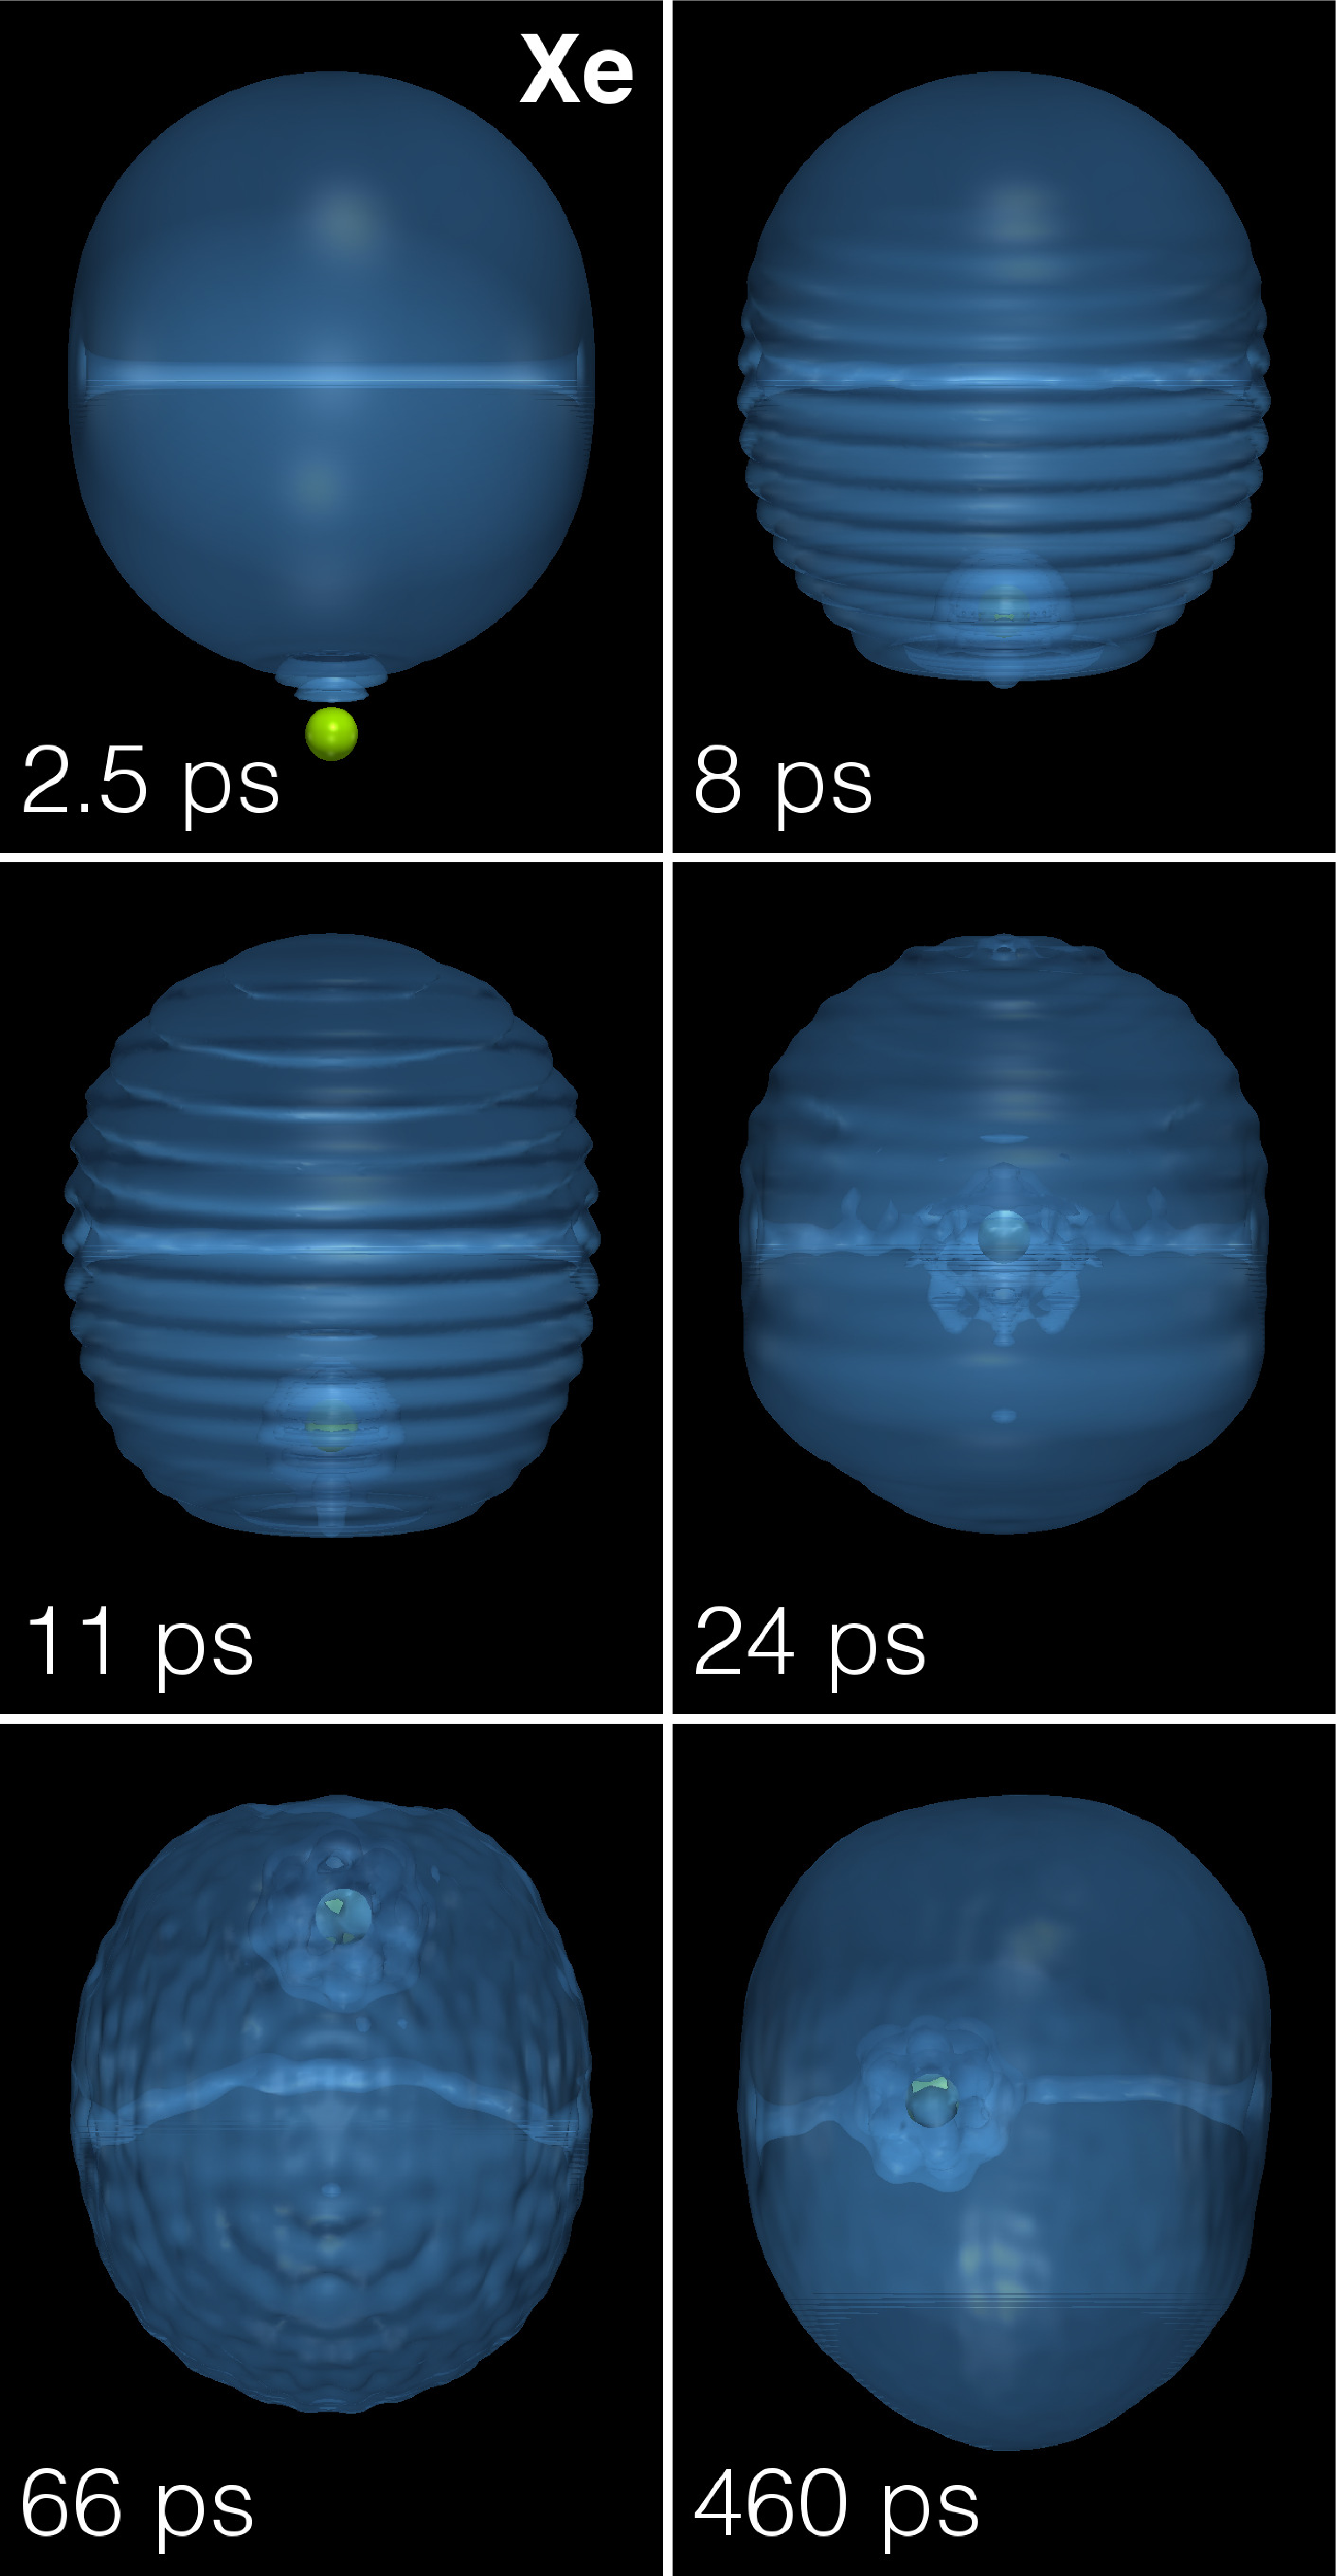
\includegraphics[width=1.0\linewidth,clip]{fig10} 
	\caption{Comparison of experimental and simulated electron binding energies. Thick solid lines: TD-DFT results. Dashed lines: Combined TD-DFT and analytical model. Thin solid lines: Biexponential fits of the experimental data.}
	\label{fig:comparePES}
\end{figure}
